
%%%%%%%%%%%%%%%%%%%%%%%%%%%%%%%%%%%%%%%%%%%%%
%%%%%%%%%%%%%% DESKRIPTIV %%%%%%%%%%%%%%%%%%%
%%%%%%%%%%%%%%%%%%%%%%%%%%%%%%%%%%%%%%%%%%%%%

	\section{Explorative Datenanalyse}		\label{descriptive}
	
	Der gesamte Mittelwert der log-transformierten Hautleitwertreaktionen in diesem Datensatz beträgt \SI{0.15}{\log\micro\siemens} ($SD=0.26$). Für die Schreckreaktion liegt der Mittelwert bei \SI{67.57}{\micro\volt} ($SD=61.94$).
	Tabelle \ref{tab:descriptive1} beinhaltet eine Übersicht über deskriptive Statistiken über den Verlauf des Akquisitionstrainings separat für beide abhängige Variablen. Eine signifikante CR (d.\,h. auf den CS+ wird bedeutend stärker reagiert als auf den CS--) ist über alle Trials hinweg für die Hautleitwertreaktionen zu beobachten und zeigt sich in den einzelnen Trials $10$ bis $14$ der zweiten Trainingshälfte. Für die Schreckreaktionen sind in Trial $12$ und $13$ die Reaktionen auf den CS+ signifikant von denen auf den CS-- verschieden sowie ebenfalls gemittelt über den Trainingszeitraum. Abbildung \ref{fig:verläufe} zeigt die durchschnittlichen Verläufe beider abhängigen Variablen über die Dauer des Akquisitionstrainings.
	Die Tabelle \ref{tab:descriptive2} zeigt bivariate Unterschiede und Zusammenhänge zwischen den abhängigen Variablen zu allen Messzeitpunkten auf. Die erste Spalte beinhaltet bivariate Korrelationen von Schreck- und Hautleitwertreaktionen (insgesamt und aufgeschlüsselt nach Messzeitpunkten). 
	\begin{table}[bth] \small \setstretch{1.5}
		\begin{threeparttable} 
			\caption{Deskriptive Statistiken \& Mittelwertunterschiede innerhalb beider abhängiger Variablen}			%ohne Punkt
			\label{tab:descriptive1}
			\begin{tabularx}{\textwidth}{lCCCCCC}  \toprule	%@{} eliminiert space zw. 2 Spalten
				\multirow[c]{2}{*}{\begin{tabular}[c]{@{}l@{}} Trial \end{tabular}} & \multicolumn{3}{c}{SCR} & \multicolumn{3}{c}{STR}	\\\cmidrule{2-7}
				& CS+\,\tnote{a}        & CS--\,\tnote{a}  & Differenz\tnote{b}   & CS+\,\tnote{a}       & CS--\,\tnote{a}   & Differenz\tnote{b}  \\\hline
				\rowcolor[HTML]{EFEFEF}
				insg. &$\mathbf{0.18\,(0.28)}$ &$\mathbf{0.12\,(0.23)}$&$\hspace*{+1.35em}\mathbf{0.06^{***}}$& $\mathbf{70.1\,(59.7)}$& $\mathbf{65.1\,(64.0)}$&$\hspace*{+0.9em}\mathbf{5.0^{**}}$   \\
				1  &$0.31\,(0.38)$ &$0.27\,(0.31)$&$0.04$& $93.1\,(61.1)$& $100.4\,(91.8)$ &$\hspace*{-0.85em}-7.3$   \\\rowcolor[HTML]{EFEFEF}
				2  &$0.14\,(0.24)$ &$0.15\,(0.23)$&$\hspace*{-0.85em}-0.01$& $92.0\,(60.6)$& $85.4\,(64.2)$ &$6.6$     \\
				3  &$0.17\,(0.21)$ &$0.15\,(0.21)$&$0.02$& $94.0\,(75.2)$& $80.5\,(60.5)$ &$13.5$      \\ \rowcolor[HTML]{EFEFEF}
				4  &$0.14\,(0.25)$ &$0.11\,(0.21)$&$0.03$& $73.2\,(55.3)$& $76.7\,(61.4)$ &$\hspace*{-0.85em}-3.5$  \\ 
				5  &$0.16\,(0.29)$ &$0.18\,(0.33)$&$\hspace*{-0.85em}-0.02$& $80.7\,(72.5)$& $83.1\,(66.1)$ &$\hspace*{-0.85em}-2.4$  \\ \rowcolor[HTML]{EFEFEF}
				6  &$0.20\,(0.31)$ &$0.18\,(0.29)$&$0.02$& $61.6\,(47.4)$& $70.4\,(75.0)$ &$\hspace*{-0.85em}-8.8$ \\
				7  &$0.08\,(0.12)$ &$0.09\,(0.17)$&$\hspace*{-0.85em}-0.01$& $66.7\,(55.6)$& $68.2\,(63.1)$ &$\hspace*{-0.85em}-1.5$  \\ \rowcolor[HTML]{EFEFEF}
				8  &$0.15\,(0.31)$ &$0.09\,(0.23)$&$0.06$& $68.1\,(56.7)$& $64.2\,(69.3)$ &$3.9$ \\ 
				9  &$0.34\,(0.43)$ &$0.26\,(0.32)$&$0.08$& $86.0\,(77.3)$& $63.2\,(67.3)$ &$\hspace*{-0.45em}22.8$ \\ \rowcolor[HTML]{EFEFEF}
				10 &$0.17\,(0.23)$ &$0.10\,(0.20)$&$\hspace*{+0.45em}0.07^{*}$& $59.1\,(49.1)$& $57.1\,(63.5)$ &$2.0$  \\ 
				11 &$0.19\,(0.26)$ &$0.06\,(0.12)$&$\hspace*{+0.9em}0.13^{**}$& $63.8\,(60.0)$& $54.2\,(56.2)$ &$9.6$ \\ \rowcolor[HTML]{EFEFEF}
				12 &$0.15\,(0.23)$ &$0.05\,(0.10)$&$\hspace*{+0.9em}0.10^{**}$& $69.1\,(60.8)$& $51.4\,(52.1)$ &$17.7^{*}$ \\ 
				13 &$0.18\,(0.28)$ &$0.05\,(0.09)$&$\hspace*{+0.9em}0.13^{**}$& $64.3\,(53.3)$& $44.5\,(38.0)$ &$\hspace*{0.45em}19.8^{**}$  \\\rowcolor[HTML]{EFEFEF}
				14 &$0.24\,(0.33)$ &$0.10\,(0.24)$&$\hspace*{+0.45em}0.14^{*}$& $47.5\,(44.9)$& $47.1\,(48.6)$ &$0.4$\\ 
				15 &$0.12\,(0.21)$ &$0.06\,(0.10)$&$0.06$& $51.7\,(45.6)$& $48.0\,(62.7)$ &$3.7$\\ \rowcolor[HTML]{EFEFEF}
				16 &$0.16\,(0.27)$ &$0.06\,(0.15)$&$0.10$& $50.4\,(49.3)$& $45.4\,(43.9)$ &$5.0$  \\[-0.2em]
				\bottomrule
			\end{tabularx}
			\begin{tablenotes}[normal, flushleft, para]
				\footnotesize{
					\item \textit{Anmerkungen.} SCR: Hautleitwertreaktion, STR: Schreckreaktion, insg.: über alle Trials hinweg.\\
					\item[a] Mittelwerte (für SCR in~\si{\log\micro\siemens}. für STR in~\si{\micro\volt}) mit Standardabweichungen in Klammern.\\
					\item[b] CS+/CS-- Differenzen; Mittelwerte auf Unterschiede getestet mittels gepaarten $t$-Tests; ${}^{*}\, p<.05$, ${}^{**}\, p<.01$, ${}^{***}\, p<.001$.}
			\end{tablenotes}
		\end{threeparttable}
	\end{table}
	Gemittelt über das ganze Training gehen höhere SCR tendenziell mit höheren Schreckreaktionen einher (kleiner Effekt von $r=.13$, $p<.001$). Auch aufgeteilt in einzelne Messzeitpunkte zeigt sich in der Tendenz ein positiver Zusammenhang zwischen den beiden Reaktionsmaßen, auch wenn er nur im ersten ($r=.25$, $p=.03$) und im neunten Trial ($r=.30$, $p=.01$) statistisch bedeutsam ist. In \nameref{appC} ist zusätzlich ein Streudiagramm zwischen den Reaktionen beider abhängiger Variablen zur Visualisierung abgebildet. 
	Die zweite Spalte der Tabelle \ref{tab:descriptive2} zeigt die Korrelationen zwischen den Differenzwerten (CS+ minus CS--) für beide Reaktionsmaße. Der insgesamt kleine, positive Zusammenhang von ($r=.15$, $p<.001$) weist darauf hin, dass eine stärkere konditionierte Reaktion auf dem einen Maß mit einer stärkeren CR auf dem anderen Maß einhergeht. Betrachtet man die einzelnen Trials ist die Korrelation zum Trial $9$ -- direkt nach der Instruktion -- positiv und signifikant ($r=.46$, $p=.004$). In Trial $3$ und $8$ sind die Korrelationen der Differenzwerte signifikant negativ. Hier gehen stärkere CR auf dem einen Maß mit geringeren  CR auf dem anderen Maß einher.
	Die letzte Spalte der bivariaten Tabelle vergleicht die Mittelwerte der CS+/CS-- Differenzen insgesamt und aufgeteilt nach Trials. Dafür wurden die Reaktionen einmalig vorab standardisiert, sodass die Differenzen als $z$-Werte vergleichbar werden. Über das ganze Akquisitionstraining hinweg unterscheiden sich die CS+/CS-- Differenzen für die beiden Maße signifikant voneinander, wobei die $z$-Differenzen der SCR im Durchschnitt größer sind als die der STR. In einzelnen Trials sind diese Unterschiede nur in Trial $14$ evident. Auch hier weist die SCR eine größere Differenz auf.
	
	Eine Überprüfung der Normalverteilung der abhängigen Variablen mittels Shapiro-Wilk-Tests \parencite{SHAPIRO1965} ergab, dass weder global noch für die einzelnen Messzeitpunkte eine Normalverteilung angenommen werden kann (\nameref{appD} liefert eine tabellarische Übersicht der Teststatistiken für beide abhängigen Variablen). Es sei darauf hingewiesen, dass dies nicht einschränkend für die Modellbildung ist. Auf eine Analyse der Ausreißer sowie der fehlenden Werte wird an dieser Stelle verzichtet, da eine Vorverarbeitung im Rahmen der Mehrebenenmodellierung nicht notwendig ist. 
	%Während der Datensatz der SCR aufgrund der automatischen Reaktionsdefinition vollständig ist, beinhaltet der Datensatz der Schreckreaktionen $13$% fehlende Werte. 
	%Eine exemplarische logistische Regression von der binären Variable \textit{fehlt} auf die Prädiktoren Trial, Versuchsperson und Stimulustyp zeigte keine signifikanten Ergebnisse, sodass angenommen werden kann, dass die Werte komplett zufällig fehlen (MCAR, engl. missing completely at random). Für eine Darstellung der Regressionsergebnisse siehe Anhang XXX.

	\begin{figure}[bht]
		\centering
		\begin{tikzpicture}[remember picture] \centering		
			\node[inner sep=0pt] (scr) at (0,0)
			{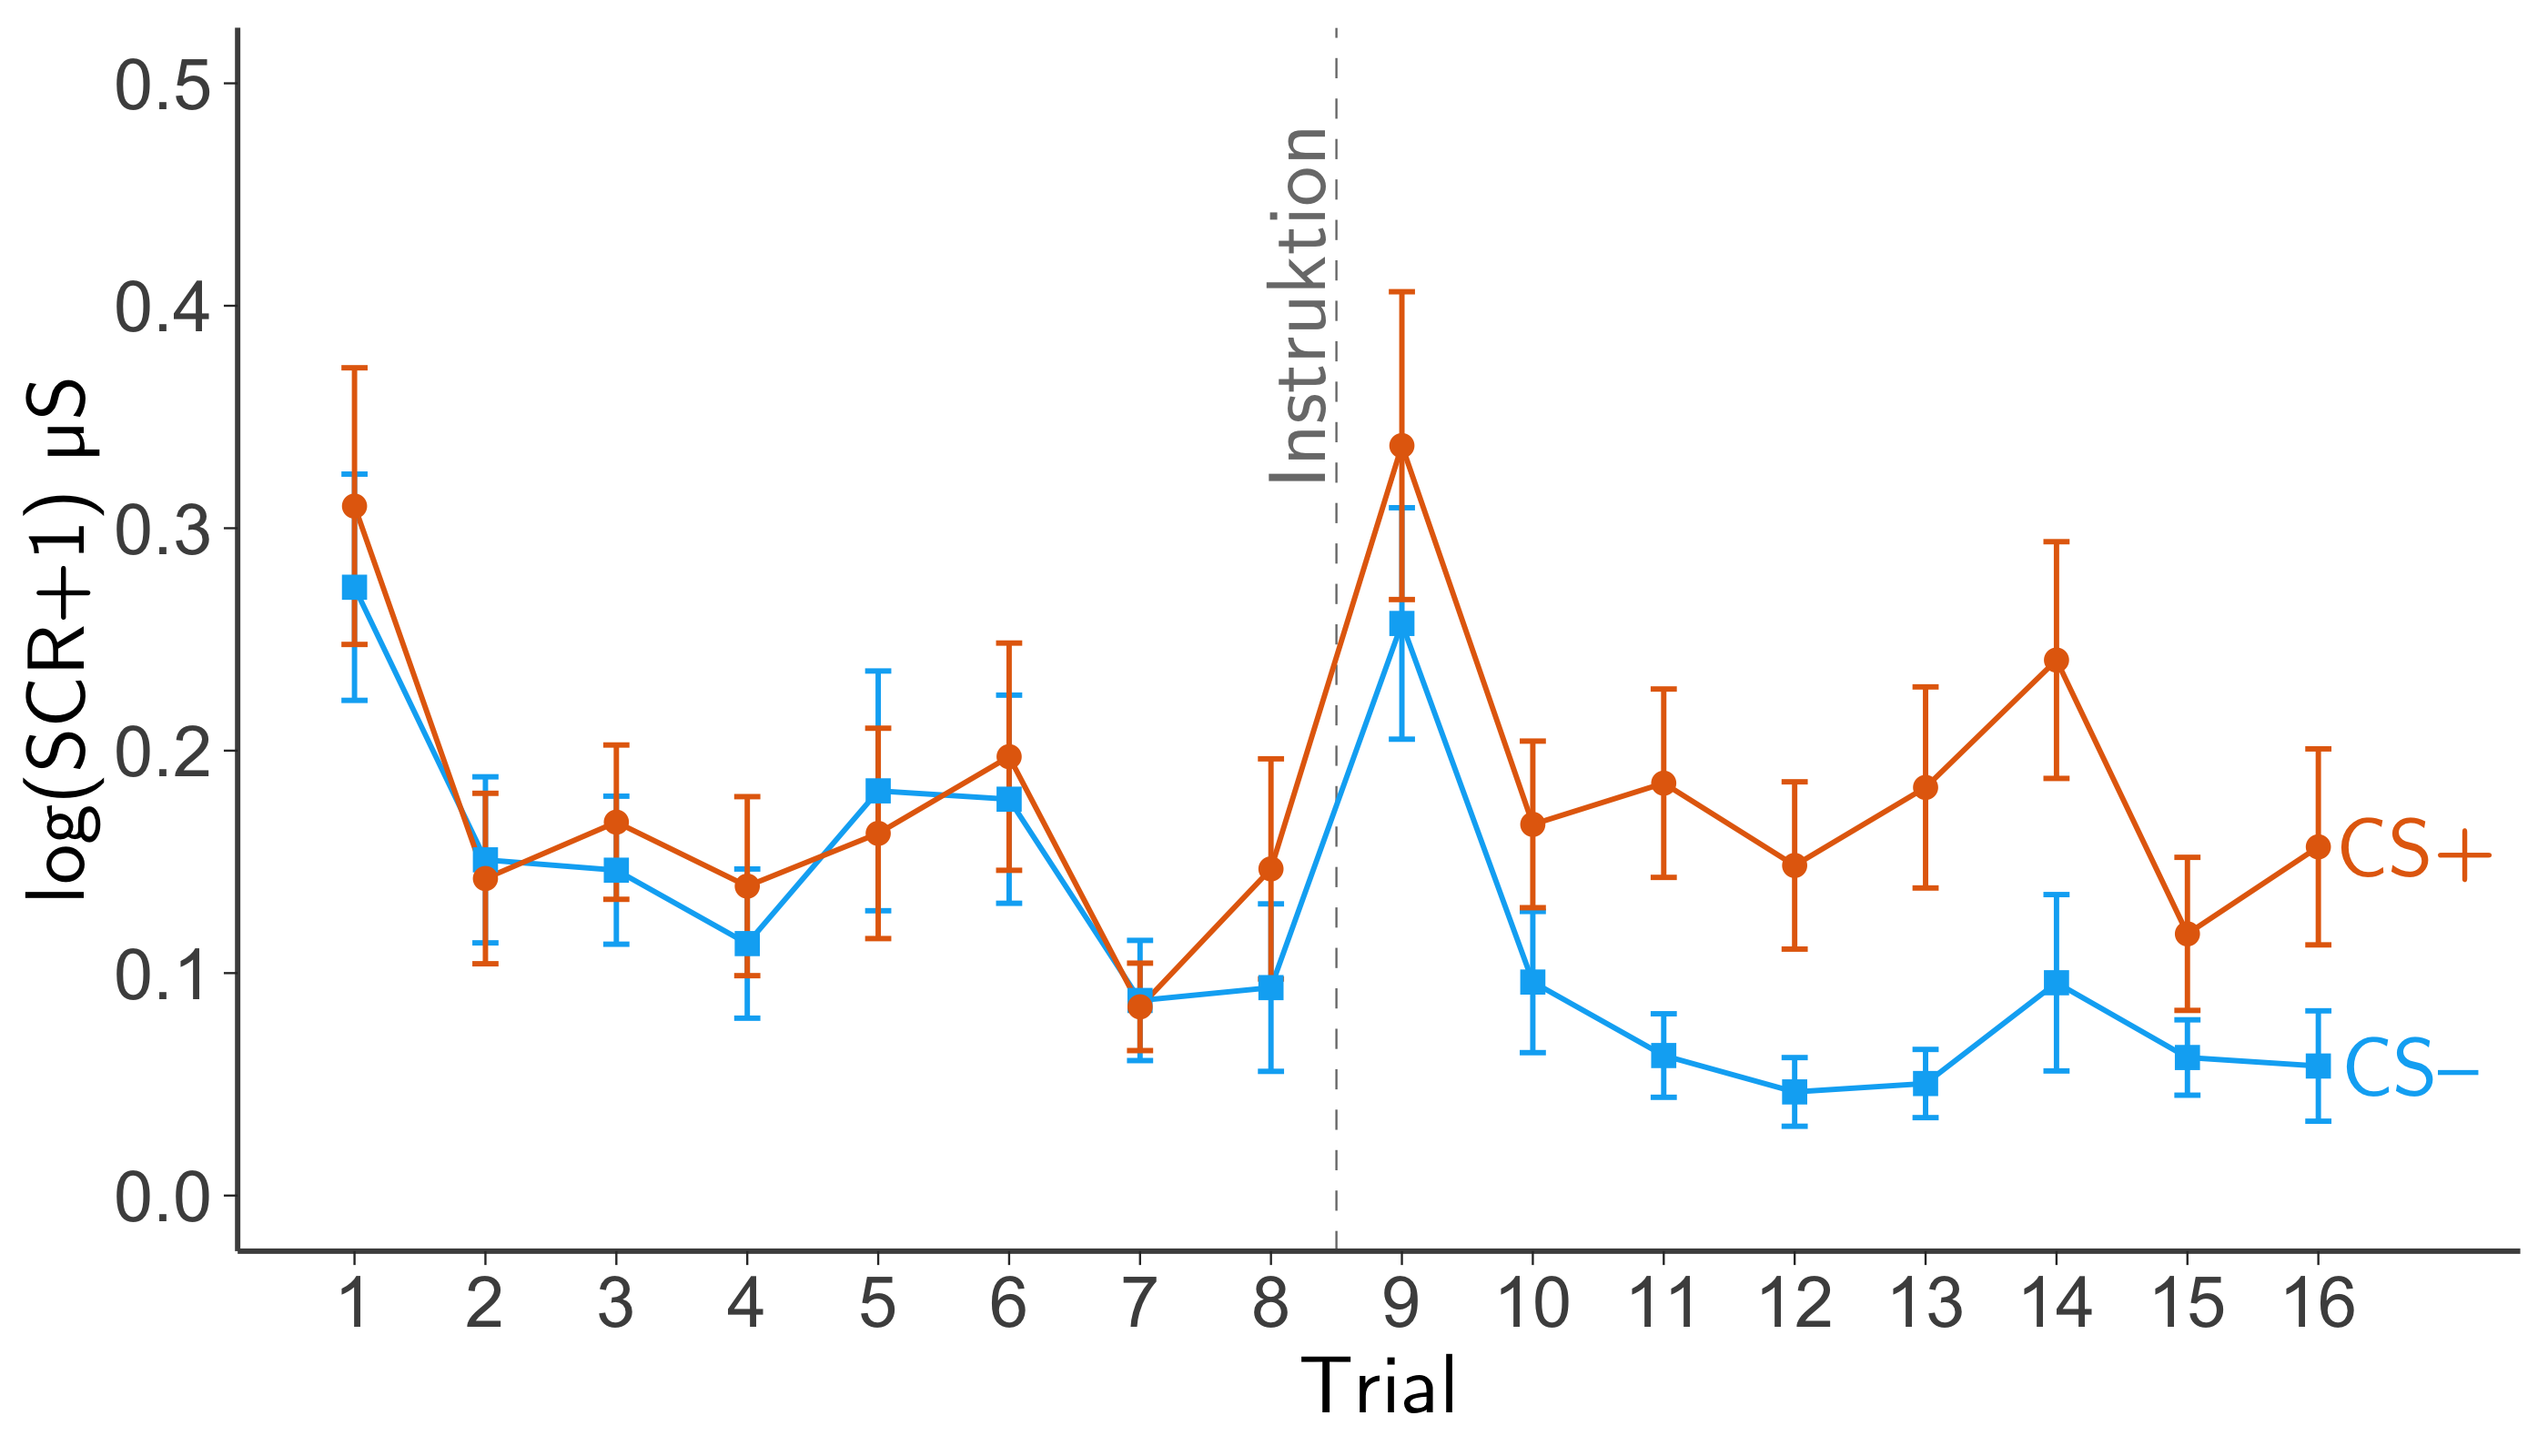
\includegraphics[scale=0.095]{scr_explor2.png}};
			\node[inner sep=0pt, below = 0.5cm of scr] (str)
			{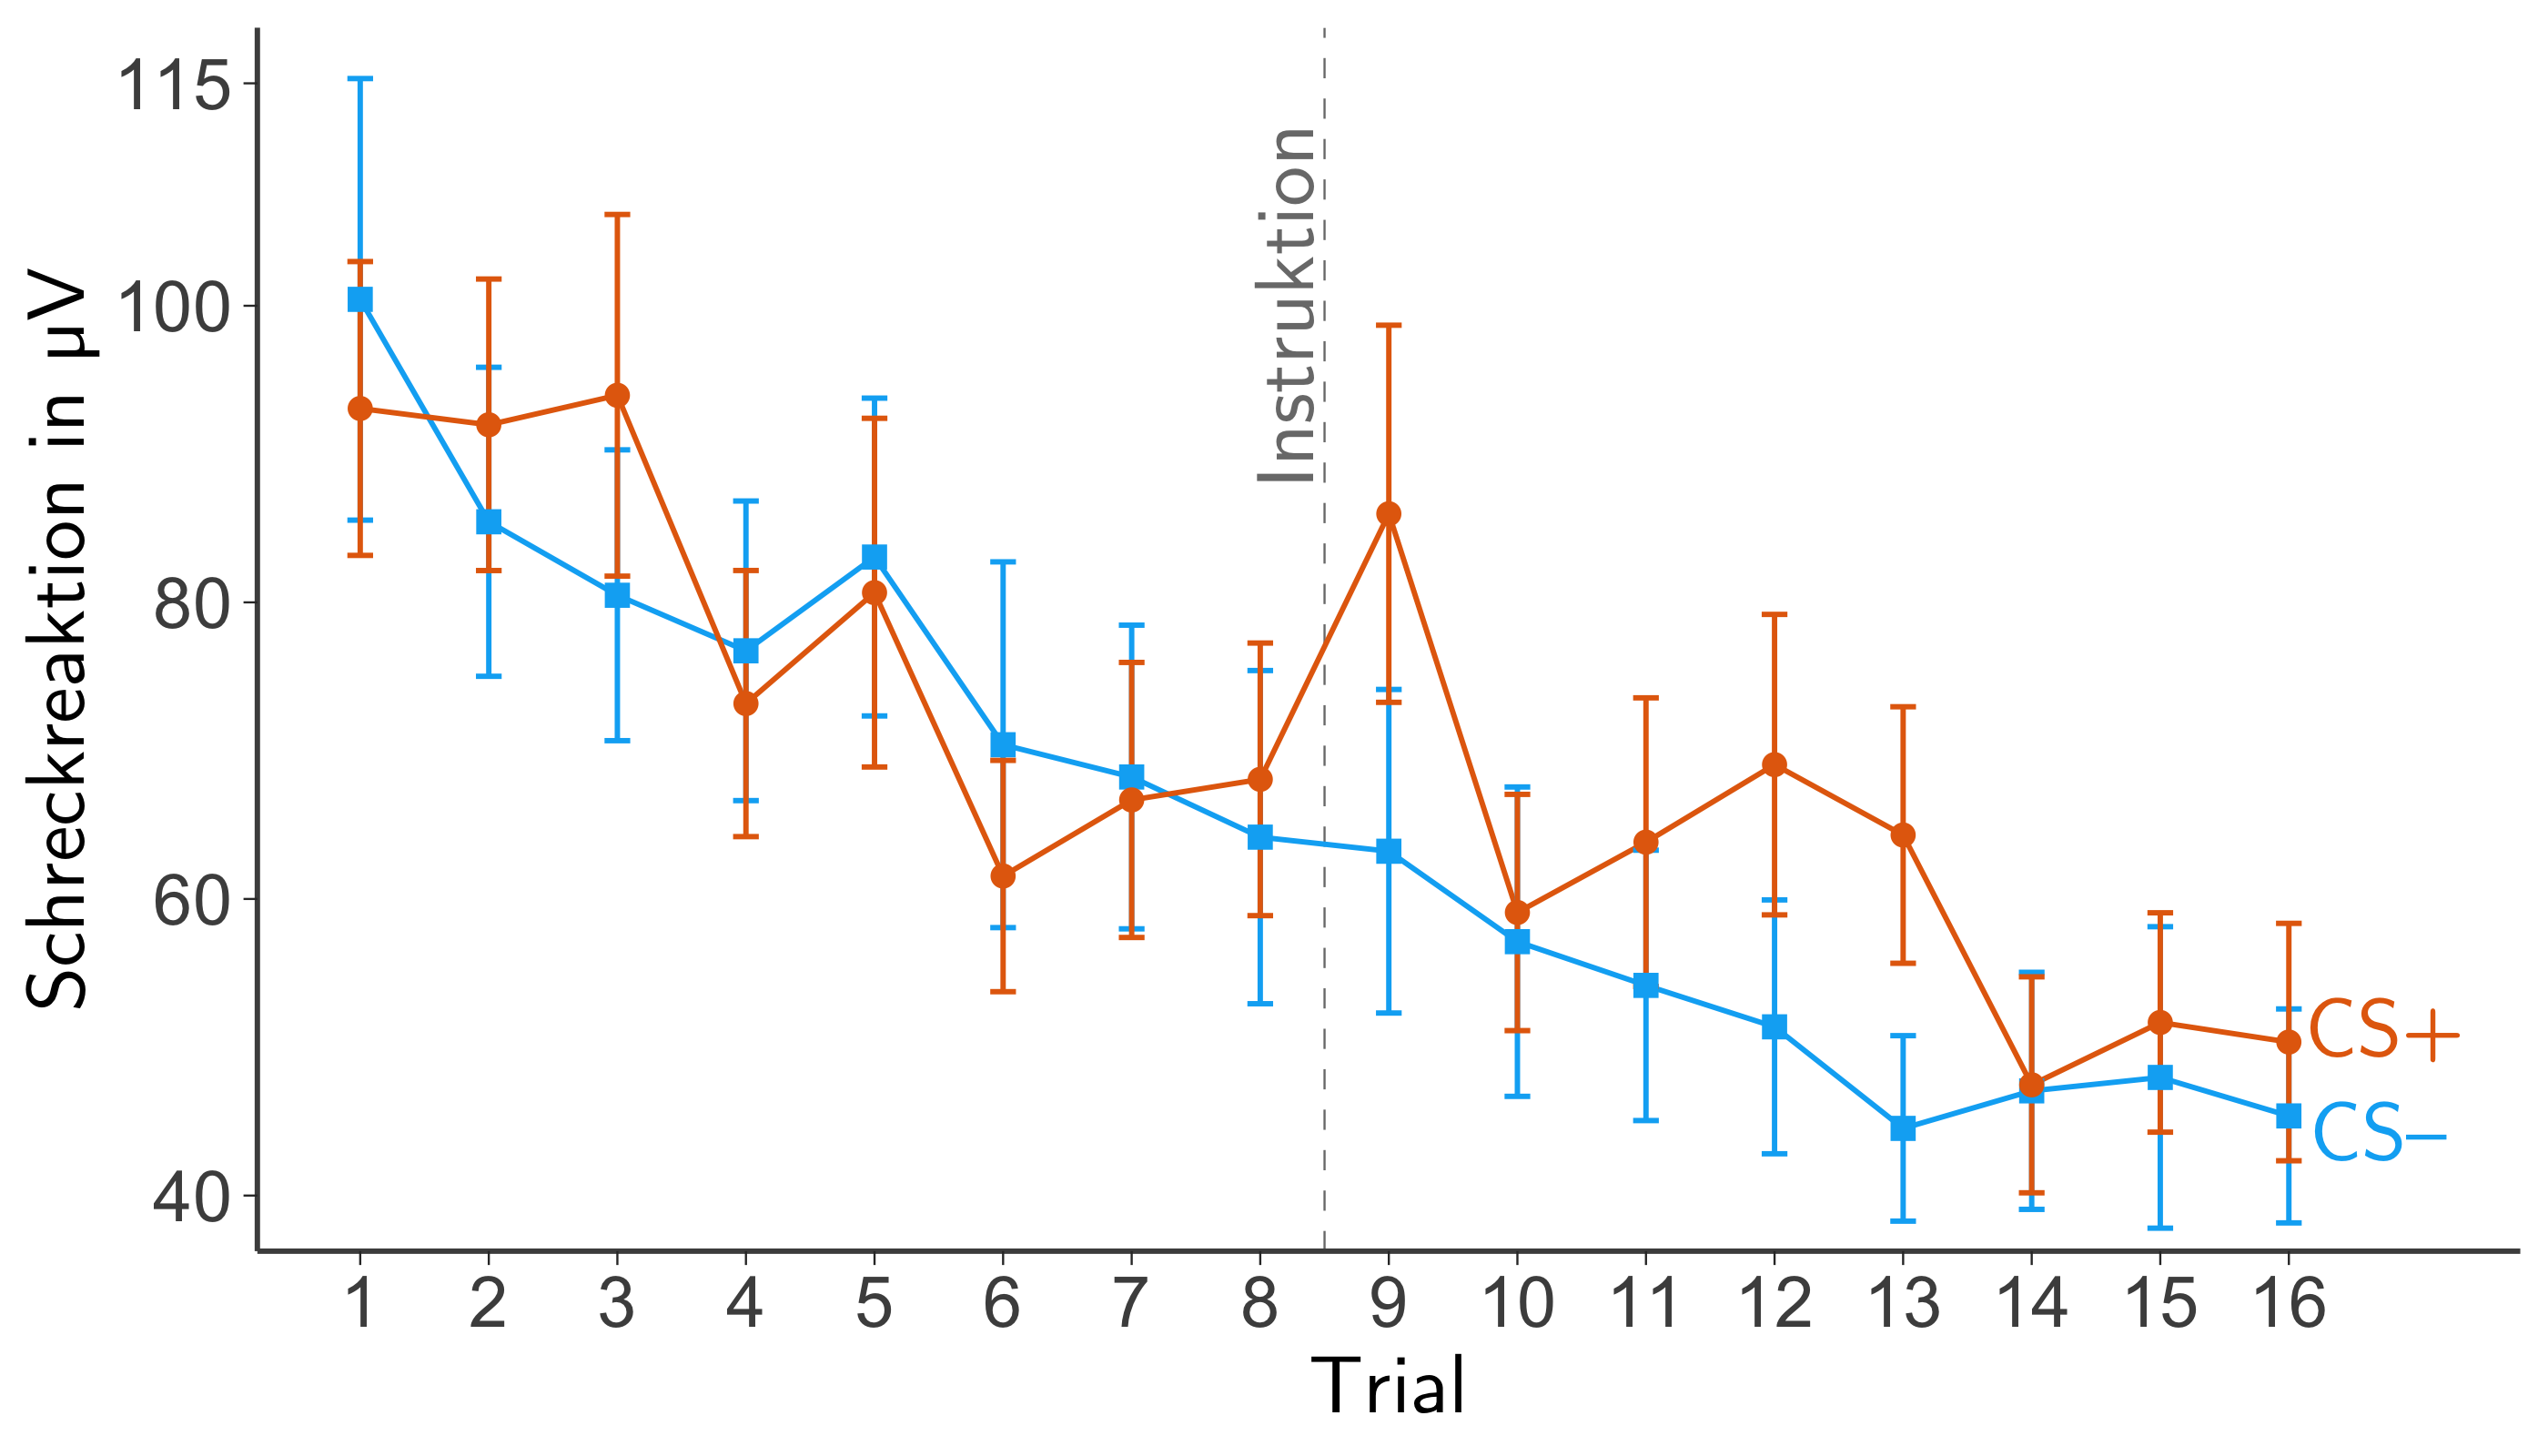
\includegraphics[scale=0.095]{str_explor2.png}};
			\node[above left = 0cm and 0.1cm of scr] (a) {\large{\textsf{\textbf{a}}}};
			\node[above left = 0cm and 0.1cm of str] (b) {\large{\textsf{\textbf{b}}}};
		\end{tikzpicture}
		\caption[Mittlere Verläufe von Hautleitwert- und Schreckreaktionen]{Mittlere Hautleitwert- (\textsf{\textbf{a}}) und Schreckreaktionen (\textsf{\textbf{b}}) auf den CS+ und CS-- über den Verlauf des Experiments. Die Fehlerbalken repräsentieren \textit{SE}.}
		\label{fig:verläufe}
	\end{figure}

	\begin{table}[tb] \small \setstretch{1.5}
	\begin{threeparttable} 
		\caption{Unterschiede \& Zusammenhänge zwischen den abhängigen Variablen}
		\label{tab:descriptive2}
		\begin{tabularx}{\textwidth}{lCCC}  \toprule	%@{} eliminiert space zw. 2 Spalten
			 \begin{tabular}[c]{@{}l@{}} Trial \end{tabular} & \begin{tabular}[c]{@{}c@{}} Korrelation zwischen \\ SCR \& STR \tnote{a}\end{tabular} & \begin{tabular}[c]{@{}c@{}} Korrelation der \\ CS+/CS-- Differenzwerte \tnote{a} \end{tabular} & \begin{tabular}[c]{@{}c@{}}$t$-Teststatistiken der\\  standardisierten Differenzwerte\tnote{b}\end{tabular} \\\hline\rowcolor[HTML]{EFEFEF}
			insg. &$\hspace*{+1.5em}\mathbf{.13^{***}}$&$\hspace*{+1.35em}\mathbf{.15^{***}}$	&$\hspace*{+0.05em}\mathbf{-2.88^{**}}$		\\
			1		&$\hspace*{+0.45em}.25^*$&$.24$		&$\hspace*{-0.85em}-1.01$		 \\\rowcolor[HTML]{EFEFEF}
			2		&$.08$		&$\hspace*{-0.85em}-.08$ 	&$0.77$		 \\
			3		&$.04$		&$\hspace*{-0.45em}-.34^{*}$ &$0.66$		 \\\rowcolor[HTML]{EFEFEF}
			4		&$.01$		&$\hspace*{-0.85em}-.02$ 	&$\hspace*{-0.85em}-0.60$		 \\
			5		&$.09$		&$.28$ 		&$0.18$		 \\\rowcolor[HTML]{EFEFEF}
			6		&$.08$		&$.28$ 		&$\hspace*{-0.85em}-0.94$		 \\
			7		&$.01$		&$\hspace*{-0.85em}-.07$ 	&$\hspace*{-0.85em}-0.22$		 \\\rowcolor[HTML]{EFEFEF}
			8		&$.04$		&$\hspace*{-0.45em}-.36^{*}$ &$\hspace*{-0.85em}-0.84$		 \\
			9		&$\hspace*{+0.9em}.30^{**}$&$\hspace*{+0.9em}.46^{**}$&$0.11$		 \\\rowcolor[HTML]{EFEFEF}
			10		&$.11$		&$.32$ 		&$\hspace*{-0.85em}-1.64$		 \\
			11		&$.06$		&$.00$ 		&$\hspace*{-0.85em}-1.60$		 \\\rowcolor[HTML]{EFEFEF}
			12		&$.16$		&$.18$ 		&$\hspace*{-0.85em}-1.07$		 	\\
			13		&$.14$		&$\hspace*{-0.85em}-.07$ 	&$\hspace*{-0.85em}-0.86$		 \\\rowcolor[HTML]{EFEFEF}
			14		&$.02$		&$.15$ 		&$\hspace*{-0.35em}-2.11^{*}$		 \\
			15		&$.08$		&$.04$ 		&$\hspace*{-0.85em}-0.91$		 \\\rowcolor[HTML]{EFEFEF}
			16		&$\hspace*{-0.85em}-.03$&$.10$ 		&$\hspace*{-0.85em}-1.37$		 \\[-0.2em]\bottomrule
		\end{tabularx}
		\begin{tablenotes}[normal, flushleft, para]
			\footnotesize{
				\item \textit{Anmerkungen.} ${}^{*}\, p<.05$, ${}^{**}\, p<.01$, ${}^{***}\, p<.001$. \item[a] Pearsons Korrelationskoeffizient $r$.	\item[b] Die Reaktionen wurden global $z$-standardisiert ($M=0$, $SD=1$) und die Differenzwerte~CS+/CS-- für SCR und STR gebildet. Diese wurden mit gepaarten~$t$-Tests auf Mittelwertunterschiede geprüft.}
		\end{tablenotes}
	\end{threeparttable}
	\end{table}	

%%%%%%%%%%%%%%%%%%%%%%%%%%%%%%%%%%%%%%%%%%%%%
%%%%%%%%%%%%%%%MODELBILDUNG%%%%%%%%%%%%%%%%%%
%%%%%%%%%%%%%%%%%%%%%%%%%%%%%%%%%%%%%%%%%%%%%

	\section{Modellbildung}		\label{modelbuild}
		Aufgrund der verhältnismäßig kleinen Stichprobengröße und der Komplexität des Modells wird über die Funktion \texttt{lmeControl} \parencite[nach][]{GRIMM2017} in R eine Kontrollfunktion definiert, die unter anderem die maximale Anzahl an Iterationen auf $500$ erhöht.
		Die Konfidenzintervalle und $p$-Werte der Modellparameter werden innerhalb des Pakets \texttt{nlme} über eine Normalapproximation der Verteilung der geschätzten Effekte berechnet \parencite[für die mathematische Herleitung siehe][]{PINHEIRO2000}.
		Eine Übersicht über den im Folgenden beschriebenen sequentiellen Modellbildungsprozess sowie über alle berechneten Modellvergleiche liefert Tabelle \ref{tab:modelbuild}. 
		
		
		\begin{table}[bth] \small \doublespacing
			\begin{threeparttable}
				\caption{Darstellung des Modellbildungsprozesses und der getätigten Modellvergleiche}			%ohne Punkt
				\label{tab:modelbuild}
				\begin{tabularx}{\textwidth}{CllCCccCCC}    \toprule%@{} eliminiert space zwischen zwei Spalten
					&  &  &  &  &  & \multicolumn{2}{c}{Anpassungsgüte} & \multicolumn{2}{c}{LRT} \\ \cmidrule{7-10}
					\multirow[t]{-2}{*}{Schritt} &
					\multirow[t]{-2}{*}{Name} &
					\multirow[t]{-2}{*}{\begin{tabular}[c]{@{}l@{}} einfacheres\\Modell\end{tabular}} &
					\multirow[t]{-2}{*}{\begin{tabular}[c]{@{}l@{}}Feste\\ Effekte\tnote{a}\end{tabular}} &
					\multirow[t]{-2}{*}{\begin{tabular}[c]{@{}l@{}}Zufällige\\ Effekte\tnote{a}\end{tabular}} &
					\multirow[t]{-2}{*}{\begin{tabular}[c]{@{}l@{}}Schätz-\\ methode\end{tabular}} & 
					logL &$df$ & $df$& $\upchi^2$  \\\midrule
					0 & null &  & $\upbeta_{00}{}^{(k)}$  &$r_{0i}{}^{(k)}$ & REML & \multicolumn{1}{l}{$-6079.4$}   & \multicolumn{1}{c}{$7$}  & \multicolumn{1}{c}{--} & \multicolumn{1}{c}{--} \\ 	
					\rowcolor[HTML]{EFEFEF}	
					1 &  ran1 & & \ditto & 
					alle & REML & \multicolumn{4}{c}{\textit{keine Konvergenz erreicht}} \\ 
					1 &  ran2 & & \ditto & $-r_{2i}{}^{(k)}$ & REML & \multicolumn{4}{c}{\textit{keine Konvergenz erreicht}} \\
					\rowcolor[HTML]{EFEFEF}		 
					1 &  ran3 & & \ditto & $-r_{1i}{}^{(k)}$ & REML & \multicolumn{4}{c}{\textit{keine Konvergenz erreicht}} \\ 
					1 &  ran4 & & \ditto & 
					$-r_{3i}{}^{(k)}$ & REML & \multicolumn{4}{c}{\textit{keine Konvergenz erreicht}} \\ 
					\rowcolor[HTML]{EFEFEF}		 
					1 &  ran5 & null & \ditto & $-r_{5i}{}^{(k)}$ & REML &
					\multicolumn{1}{l}{$-5976.4$} & \multicolumn{1}{c}{$14$}  & \multicolumn{1}{c}{$7$} & \multicolumn{1}{l}{$~~206^{***}$} \\\hline	 
					2 & time1 &  ran5\tnote{b} & $+\upbeta_{10}{}^{(k)}$  &
					\begin{tabular}[c]{@{}l@{}}$r_{0i}{}^{(k)}$\\ $r_{4i}{}^{(k)}$\end{tabular}  & ML &
					\multicolumn{1}{l}{$-5934.3$} & \multicolumn{1}{c}{$16$}  & \multicolumn{1}{c}{$2$} & \multicolumn{1}{l}{$84.25^{***}$} \\ 
					\rowcolor[HTML]{EFEFEF}		
					2 & time2 & time1 & $+\upbeta_{20}{}^{(k)}$ & \ditto  & ML &
					\multicolumn{1}{l}{$-5931.5$} & \multicolumn{1}{c}{$18$}  & \multicolumn{1}{c}{$2$} & \multicolumn{1}{l}{$~5.59$} \\ 
					2 & time2.1 & time1 & $-\upbeta_{20}{}^{(1)}$ & \ditto  & ML &
					\multicolumn{1}{l}{$-5931.9$} & \multicolumn{1}{c}{$17$}  & \multicolumn{1}{c}{$1$} & \multicolumn{1}{l}{$~4.86^{*}$} \\
					\rowcolor[HTML]{EFEFEF}	
					3 & cs1 & time2.1 & $+\upbeta_{30}{}^{(k)}$ &\ditto  & ML &
					\multicolumn{1}{l}{$-5917.0$} & \multicolumn{1}{c}{$19$}  & \multicolumn{1}{c}{$2$} & \multicolumn{1}{l}{$29.68^{***}$} \\
					3 & cs2 & cs1 & $+\upbeta_{40}{}^{(k)}$ & \ditto  & ML &
					\multicolumn{1}{l}{$-5911.3$} & \multicolumn{1}{c}{$21$}  & \multicolumn{1}{c}{$2$} & \multicolumn{1}{l}{$11.36^{**}$} \\
					\rowcolor[HTML]{EFEFEF}	
					3 & cs2.1 & cs1 & $-\upbeta_{40}{}^{(2)}$ & \ditto  & ML &
					\multicolumn{1}{l}{$-5912.6$} & \multicolumn{1}{c}{$20$}  & \multicolumn{1}{c}{$1$} & \multicolumn{1}{l}{$~8.93^{**}$} \\ 
					3 & cs3 & cs2.1 & $+\upbeta_{50}{}^{(k)}$ &
					\ditto  & ML &
					\multicolumn{1}{l}{$-5911.9$} & \multicolumn{1}{c}{$22$}  & \multicolumn{1}{c}{$2$} & \multicolumn{1}{l}{$~1.25$} \\ %\hline
					\rowcolor[HTML]{EFEFEF}	
					& fin & -- & $-\upbeta_{50}{}^{(k)}$ &
					\ditto  & REML &
					\multicolumn{1}{l}{$-5927.0$} & \multicolumn{1}{c}{$20$}  & \multicolumn{1}{c}{--} & \multicolumn{1}{c}{--} \\ [-0.2em]
					\bottomrule
				\end{tabularx}
				\begin{tablenotes}[normal, flushleft, para]
					\footnotesize{
						\item \textit{Anmerkungen.} $N=2419$ Reaktionen (Ebene~1), $n=38$ Versuchspersonen (Ebene~2); LRT: Likelihood-Ratio Test ggü. einfacherem Modell mit ${}^{*}\, p<.05$, ${}^{**}\, p<.01$, ${}^{***}\, p<.001$; $df$: Freiheitsgrade.\\
						\item[a] bei positivem Vorzeichen wird dieser Term in diesem Schritt zum Modell hinzugefügt; bei negativen Vorzeichen wird er entfernt; Terme ohne Vorzeichen beschreiben die aktuelle, vollständige Struktur.
						\item[b] für den Vergleich erneut mit ML-Verfahren geschätzt.}
				\end{tablenotes}
			\end{threeparttable}
		\end{table}
	
		%null
			Das in Schritt~0 erstellte Nullmodell (Modellname \textit{null}) schätzt einen Intercept für die Hautleitwertreaktion von \SI{0.15}{\log\micro\siemens} ($\upbeta_{00}{}^{(1)}$, $SE=0.022$, Konfidenzintervall $KI\,\left[0.108,0.194\right]$). Für die Schreckreaktion beträgt die Schätzung \SI{67.19}{\micro\volt} ($\upbeta_{00}{}^{(2)}$, $SE=8.14$, $KI\,\left[51.24,83.13\right]$). 
			Die zufälligen Effekte zeigen mit einer Standardabweichung von $0.13$ für die SCR ($KI\,\left[0.101; 0.166\right]$) und $49.7$ für die Schreckreaktion ($KI\,\left[39.5; 62.5\right]$) substanzielle Varianz der Versuchspersonen in ihren Intercepts auf den jeweiligen Reaktionsvariablen.		
			
		%random1
			In Schritt 1 wird das Nullmodell in seiner zufälligen Effekt-Struktur auf den maximal möglichen Aufbau wie in Gleichung \eqref{eq:matrix2} erweitert (Modellname \textit{ran1}). 
			Dieses Modell konvergiert mit den hier verwendeten Daten nicht, sodass pragmatische Entscheidungen zur Reduzierung der Komplexität getroffen wurden. 
			Lose orientiert an den Empfehlungen von \textcite{BRAUER2018} wird die Struktur der zufälligen Effekte sequentiell reduziert -- zunächst, bis Konvergenz erzielt wird.
			Wenn die Interaktion von sogenannten \textit{within-subject} Prädiktoren (innerhalb Versuchspersonen) von Interesse ist, soll diese laut \textcite{BARR2013} nach Möglichkeit zufällig modelliert und einfachere zufällige Effekte fallen gelassen werden. Die Entscheidungen werden daher im Sinne der Untersuchung des Furchtlernens getroffen, für das insbesondere die Interaktion \textit{CS$\times$lin} (sprich die Differenzierung der Stimuli über die Zeit) wichtig ist. Unter dieser Begründung sind die Entscheidungen zur zufälligen Effektstruktur sowohl daten- als auch theoriegetrieben.
			Zunächst wird auf den zufälligen Effekt von \textit{quad} $\left(r_{2i}{}^{(k)}\right)$ für beide abhängigen Variablen verzichtet.
		%random2
			Nachdem auch dieses Modell keine Konvergenz erreicht, wird der zufällige Slope für den linearen Zeitterm $\left(r_{1i}{}^{(k)}\right)$ entfernt,
		%random3
			%Hierbei ergab sich ein rechnerischer Fehler: Unable to form Cholesky decomposition: the leading minor of order 7 is not pos.def.
			doch auch dann konvergiert das Modell nicht.
		%random4 & random5
			Erst ein zusätzliches Herausnehmen des zufälligen Anstiegs für den Stimulustyp $\left( r_{3i}{}^{(k)}\right)$ und seine Interaktion mit dem quadratischen Zeitterm $\left( r_{5i}{}^{(k)}\right)$ führen zur Konvergenz des Modells.
			Übrig bleiben für die Struktur der zufälligen Effekte also der Intercept $\left(r_{0i}{}^{(k)}\right)$ und die Interaktion \textit{CS$\times$lin} $\left(r_{4i}{}^{(k)}\right.$; Modellname \textit{ran5}$\left. \right)$.
			%Brauer et al.:
				%1. log-Transformation der Schreckreaktion
				%2. Check whether the nonconvergence is due to the presence of a few subjects (or items) with a small number of observations in particular cells. If yes, consider imputing data or removing the problematic subjects (or items).
				%3. If you have a design with two within-unit predictors and your hypothesis concerns the interaction, remove the by-unit random slopes for the within-unit predictors and the lower-order interactions, but do not remove the by-unit random slope for the highest-order interaction(s) between the within-unit predictors (Barr, 2013, Frontiers).
				%4. Selectively remove covariances among random effects: Start out by removing covariances of predictors that are not directly related to your hypotheses (X3 and X4 mentioned in remedy #12 if you have decided to keep these predictors in the model). Continue to remove covariances that you suspect to be close to zero anyway. Finally, remove all covariances among random effects.
		
		%time1
			Im nächsten Schritt wird die Struktur der Zeitterme gewählt. 
			Für beide abhängigen Variablen zeigen sich die linearen Terme als signifikante Prädiktoren (SCR: $\upbeta_{10}{}^{(1)}=-0.007$, $SE=0.002$, $p<.001$; STR: $\upbeta_{10}{}^{(2)}=-3.22$, $SE=0.35$, $p<.001$). Ein LRT zeigt, dass die Hinzunahme die Anpassungsgüte deutlich verbessert ($\upchi^2(2)=84.25$, $p<.001$). 
		%time2
			Bei den quadratischen Zeittermen zeichnet sich ein heterogeneres Bild ab. Für die SCR ist der neue Term kein signifikanter Prädiktor ($\upbeta_{20}{}^{(1)}=0.0003$,  $p=.39$), wohl aber für die Schreckreaktion ($\upbeta_{20}{}^{(2)}=0.109$,  $SE=0.05$, $p=.028$). 
			Der quadratische Zeitterm wird daher für die SCR aus dem Modell entfernt (Modellname \textit{time2.1}).
			Ein anschließender LRT zeigt, dass das Hinzufügen von \textit{quad} für die Schreckreaktion die Anpassungsgüte gegenüber dem Modell mit nur linearen festen Effekten verbessert ($\upchi^2(1)=4.86$, $p=.028$).
			
		%cs1
			Nach der Festlegung der Zeitstruktur wird in Schritt 3 der Prädiktor Stimulustyp in das Modell aufgenommen. 
			Für beide abhängige Variablen ist der einfache \textit{CS}-Term signifikant (SCR: $\upbeta_{30}{}^{(1)}=0.058$, $SE=0.0124$, $p<.001$; 
			STR: $\upbeta_{30}{}^{(2)}=	5.19$, $SE=1.866$, $p=.005$). 
			Die Anpassungsgüte dieses Modells (Modellname \textit{cs1}) gegenüber dem einfacheren (\textit{time2.1}) ist bedeutend besser ($\upchi^2(2)=29.68$, $p<.001$). 
		%cs2 and cs2.1
			Als nächstes wird nun auch der feste Effekt der Interaktion vom Stimulustyp mit dem linearen Term eingefügt. Prinzipiell verbessert das Hinzufügen dieses festen Effekts die Anpassungsgüte des Modells ($\upchi^2(2)=11.36$, $p=.003$). Betrachtet man die beiden abhängigen Variablen separat voneinander, zeigt sich, dass die Interaktion nur für die SCR signifikant ist ($\upbeta_{40}{}^{(1)}=0.0084$, $SE=0.0029$, $p=.004$), nicht aber für die Schreckreaktion ($\upbeta_{40}{}^{(2)}=0.713$, $SE=0.457$, $p=.119$). Für letztere wird der Term daher im Sinne der Sparsamkeit entfernt (Modellname \textit{cs2.1}). 
		%cs3
			Das Hinzufügen der Interaktion \textit{CS$\times$quad} als festen Effekt ist für keine der abhängigen Variablen von Bedeutung (SCR: $\upbeta_{50}{}^{(1)}=0.0002$, $p=.41$; STR: $\upbeta_{50}{}^{(2)}=-0.074$, $p=.46$) und verbessert auch die Anpassungsgüte nicht ($\upchi^2(2)=1.25$, $p=.536$). Demnach wird diese nicht in das finale Modell mit aufgenommen.
		
				
%%%%%%%%%%%%%%%%%%%%%%%%%%%%%%%%%%%%%%%%%%%%%
%%%%%%%%%%%%%%FINALES MODEL%%%%%%%%%%%%%%%%%%
%%%%%%%%%%%%%%%%%%%%%%%%%%%%%%%%%%%%%%%%%%%%%	
	\section{Das finale Modell}		\label{finalmodel}
		
		Das finale multivariate Wachstumsmodell wird für die Schreckreaktionen mit Polynomen ersten und zweiten und für die Hautleitwertreaktion nur mit Polynomen ersten Grades modelliert. Es enthält feste Effekte für den Stimulustyp mit dem CS-- als Referenzkategorie sowie eine Interaktion von \textit{CS$\times$lin} für die SCR.		
		Die Struktur der zufälligen Effekte für die Versuchspersonen besteht aus zufälligen Intercepts und der als zufällig modellierten Interaktion \textit{CS$\times$lin} für beide Reaktionsmaße.
		Das final aufgestellte Modell kann als Teilmenge des maximalen Modells aus Gleichung \eqref{eq:matrix2} beschrieben werden mit analoger Notation:
			\begin{align*}
				\mat{B}^{(k)} = \begin{bmatrix} \upbeta_{00}{}^{(k)} \\ \upbeta_{10}{}^{(k)} \\\upbeta_{20}{}^{(2)}\\\upbeta_{30}{}^{(k)}\\\upbeta_{40}{}^{(1)}\end{bmatrix}, \qquad		
				\mat{X}_1 = \begin{bmatrix}1\\ \text{lin}_{it}\\ \text{quad}_{it}\\ \text{CS}_{it}\\ \text{CS}_{it}\times\text{lin}_{it}\end{bmatrix}, \qquad
				\mat{R}^{(k)} = \begin{bmatrix} r_{0i}{}^{(k)} \\ r_{4i}{}^{(k)} 
				\end{bmatrix}, \qquad
				\mat{X}_2 = \begin{bmatrix}1\\ \text{CS}_{it}\times\text{lin}_{it}
				\end{bmatrix}
				\nr\label{eq:final1}
			\end{align*}
			\begin{align*}
				y_{it}{}^{(k)}= \sum_{m=1}^{2}\, \updelta_m \,\left[ 
				\left(\mat{B}^{(m)}\right)^T\mat{X}_1+
				\left(\mat{R}^{(m)}\right) ^T\mat{X}_2+
				e_{it}{}^{(m)}\right] 
				\nr\label{eq:final2}
			\end{align*}

		Die auf Basis des Modells vorhergesagten Verläufe für beide Reaktionsmaße sind in Abb. \ref{fig:predict} verdeutlicht.
		Tabelle \ref{tab:final} zeigt die Ergebnisse des finalen Modells, darunter die Schätzungen, Standardfehler und Konfidenzintervalle der festen Parameter, die im finalen Modell enthalten sind.
		Für die Hautleitwertreaktion beträgt der geschätzte Intercept \SI{0.065}{\log\micro\siemens} ($SE=0.029$). Er beschreibt die durchschnittliche Höhe der Reaktion auf den CS-- genau in der Mitte des Akquisitionstrainings.
		Diese mittlere Reaktion variiert substanziell zwischen Versuchspersonen mit einer Standardabweichung von $0.13$ rings um den Gesamt-Intercept (zufälliger Intercept). 
		Abbildung \ref{fig:randomeffects} zeigt die Intercepts der Versuchspersonen als absolute Werte (\ref{fig:randomeffects}a) und als Abweichungen in Standardabweichungen skaliert vom Gesamt-Intercept (\ref{fig:randomeffects}c). Hier wird deutlich, dass für ca. ein Drittel der Versuchspersonen negative Intercepts vom Modell vorhergesagt werden.
		Die SCR werden durch lineare Wachstumskurven modelliert, wobei sie im Mittel über den Verlauf des Akquisitionstrainings um \SI{0.018}{\log\micro\siemens} abnehmen ($SE=0.004$).
		Der Stimulustyp hat einen signifikanten Einfluss auf die Höhe der SCR. Die Reaktionen auf den CS+ sind durchschnittlich \SI{0.058}{\log\micro\siemens} höher als auf den CS-- ($SE=0.012$).
		Für die Interaktion zwischen Stimulustyp und linearem Term schätzt das Modell eine Slope von $0.009$ ($\upbeta_{40}{}{(1)}$, $SE=0.003$).
		\begin{figure}[bh]
			\centering
			\begin{tikzpicture}[remember picture] \centering		
				\node[inner sep=0pt] (scr) at (2,0)
				{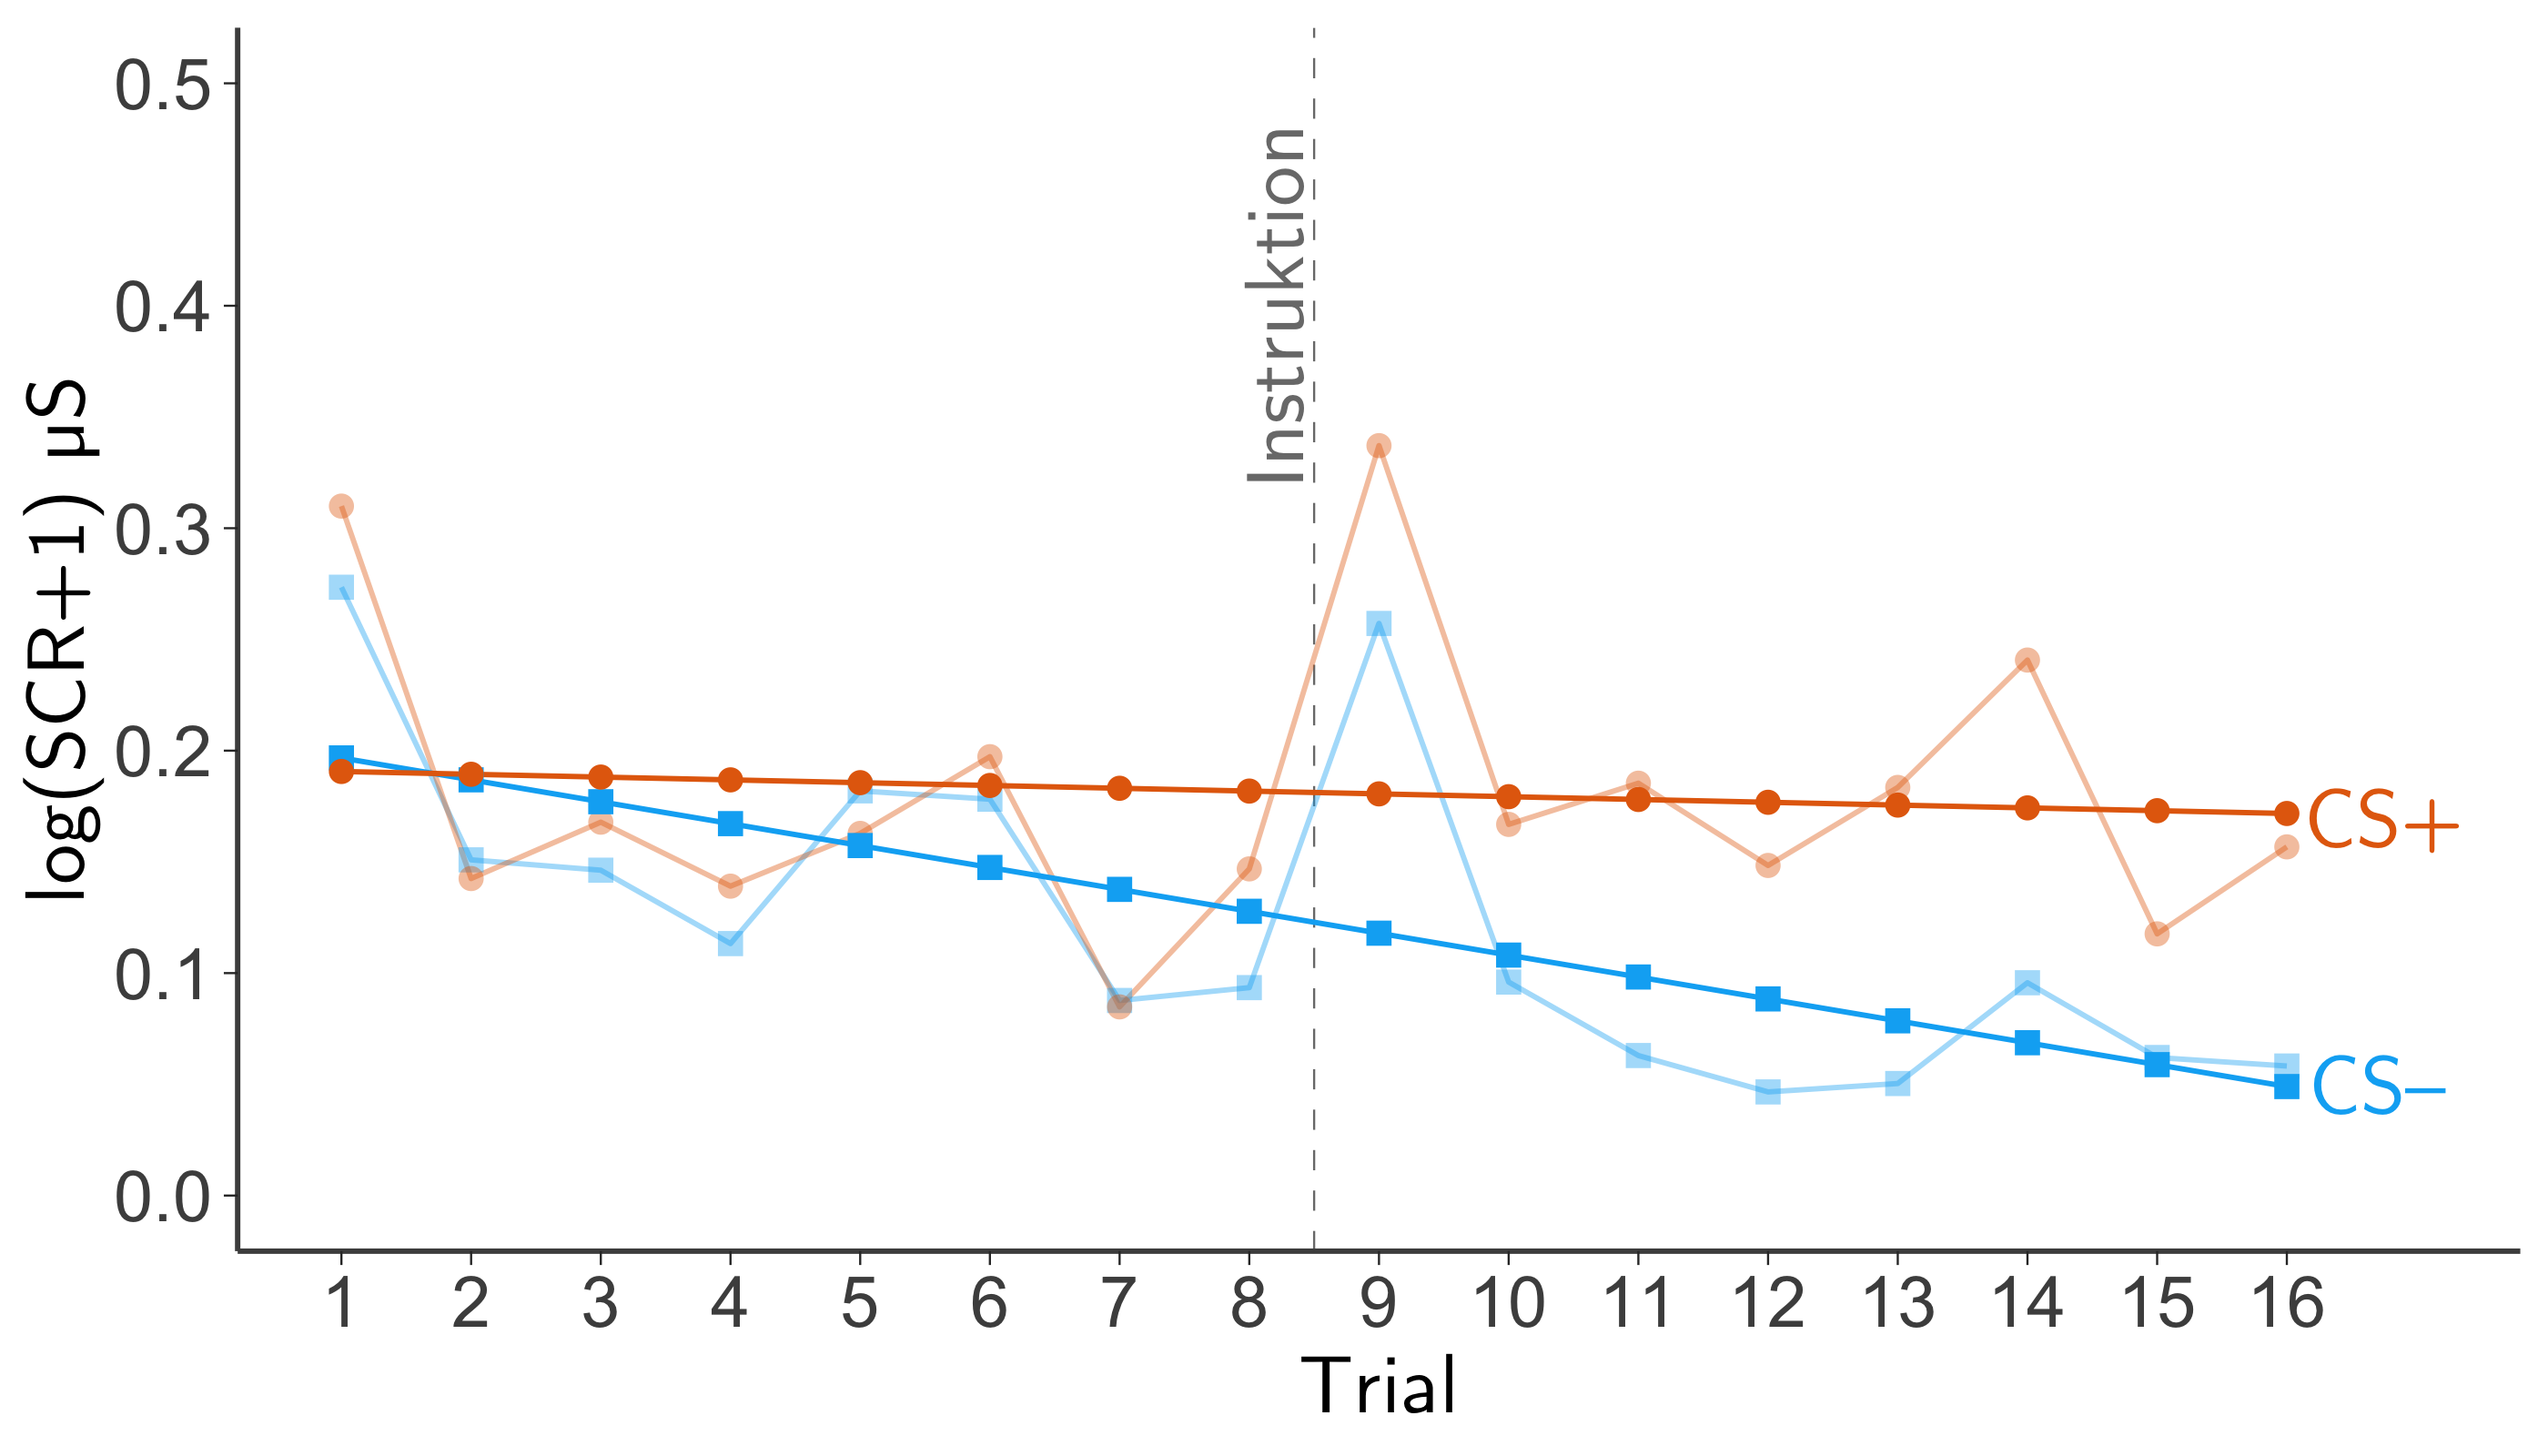
\includegraphics[scale=0.10]{fit_scr.png}};
				\node[inner sep=0pt] (str) at (2,-6.5)
				{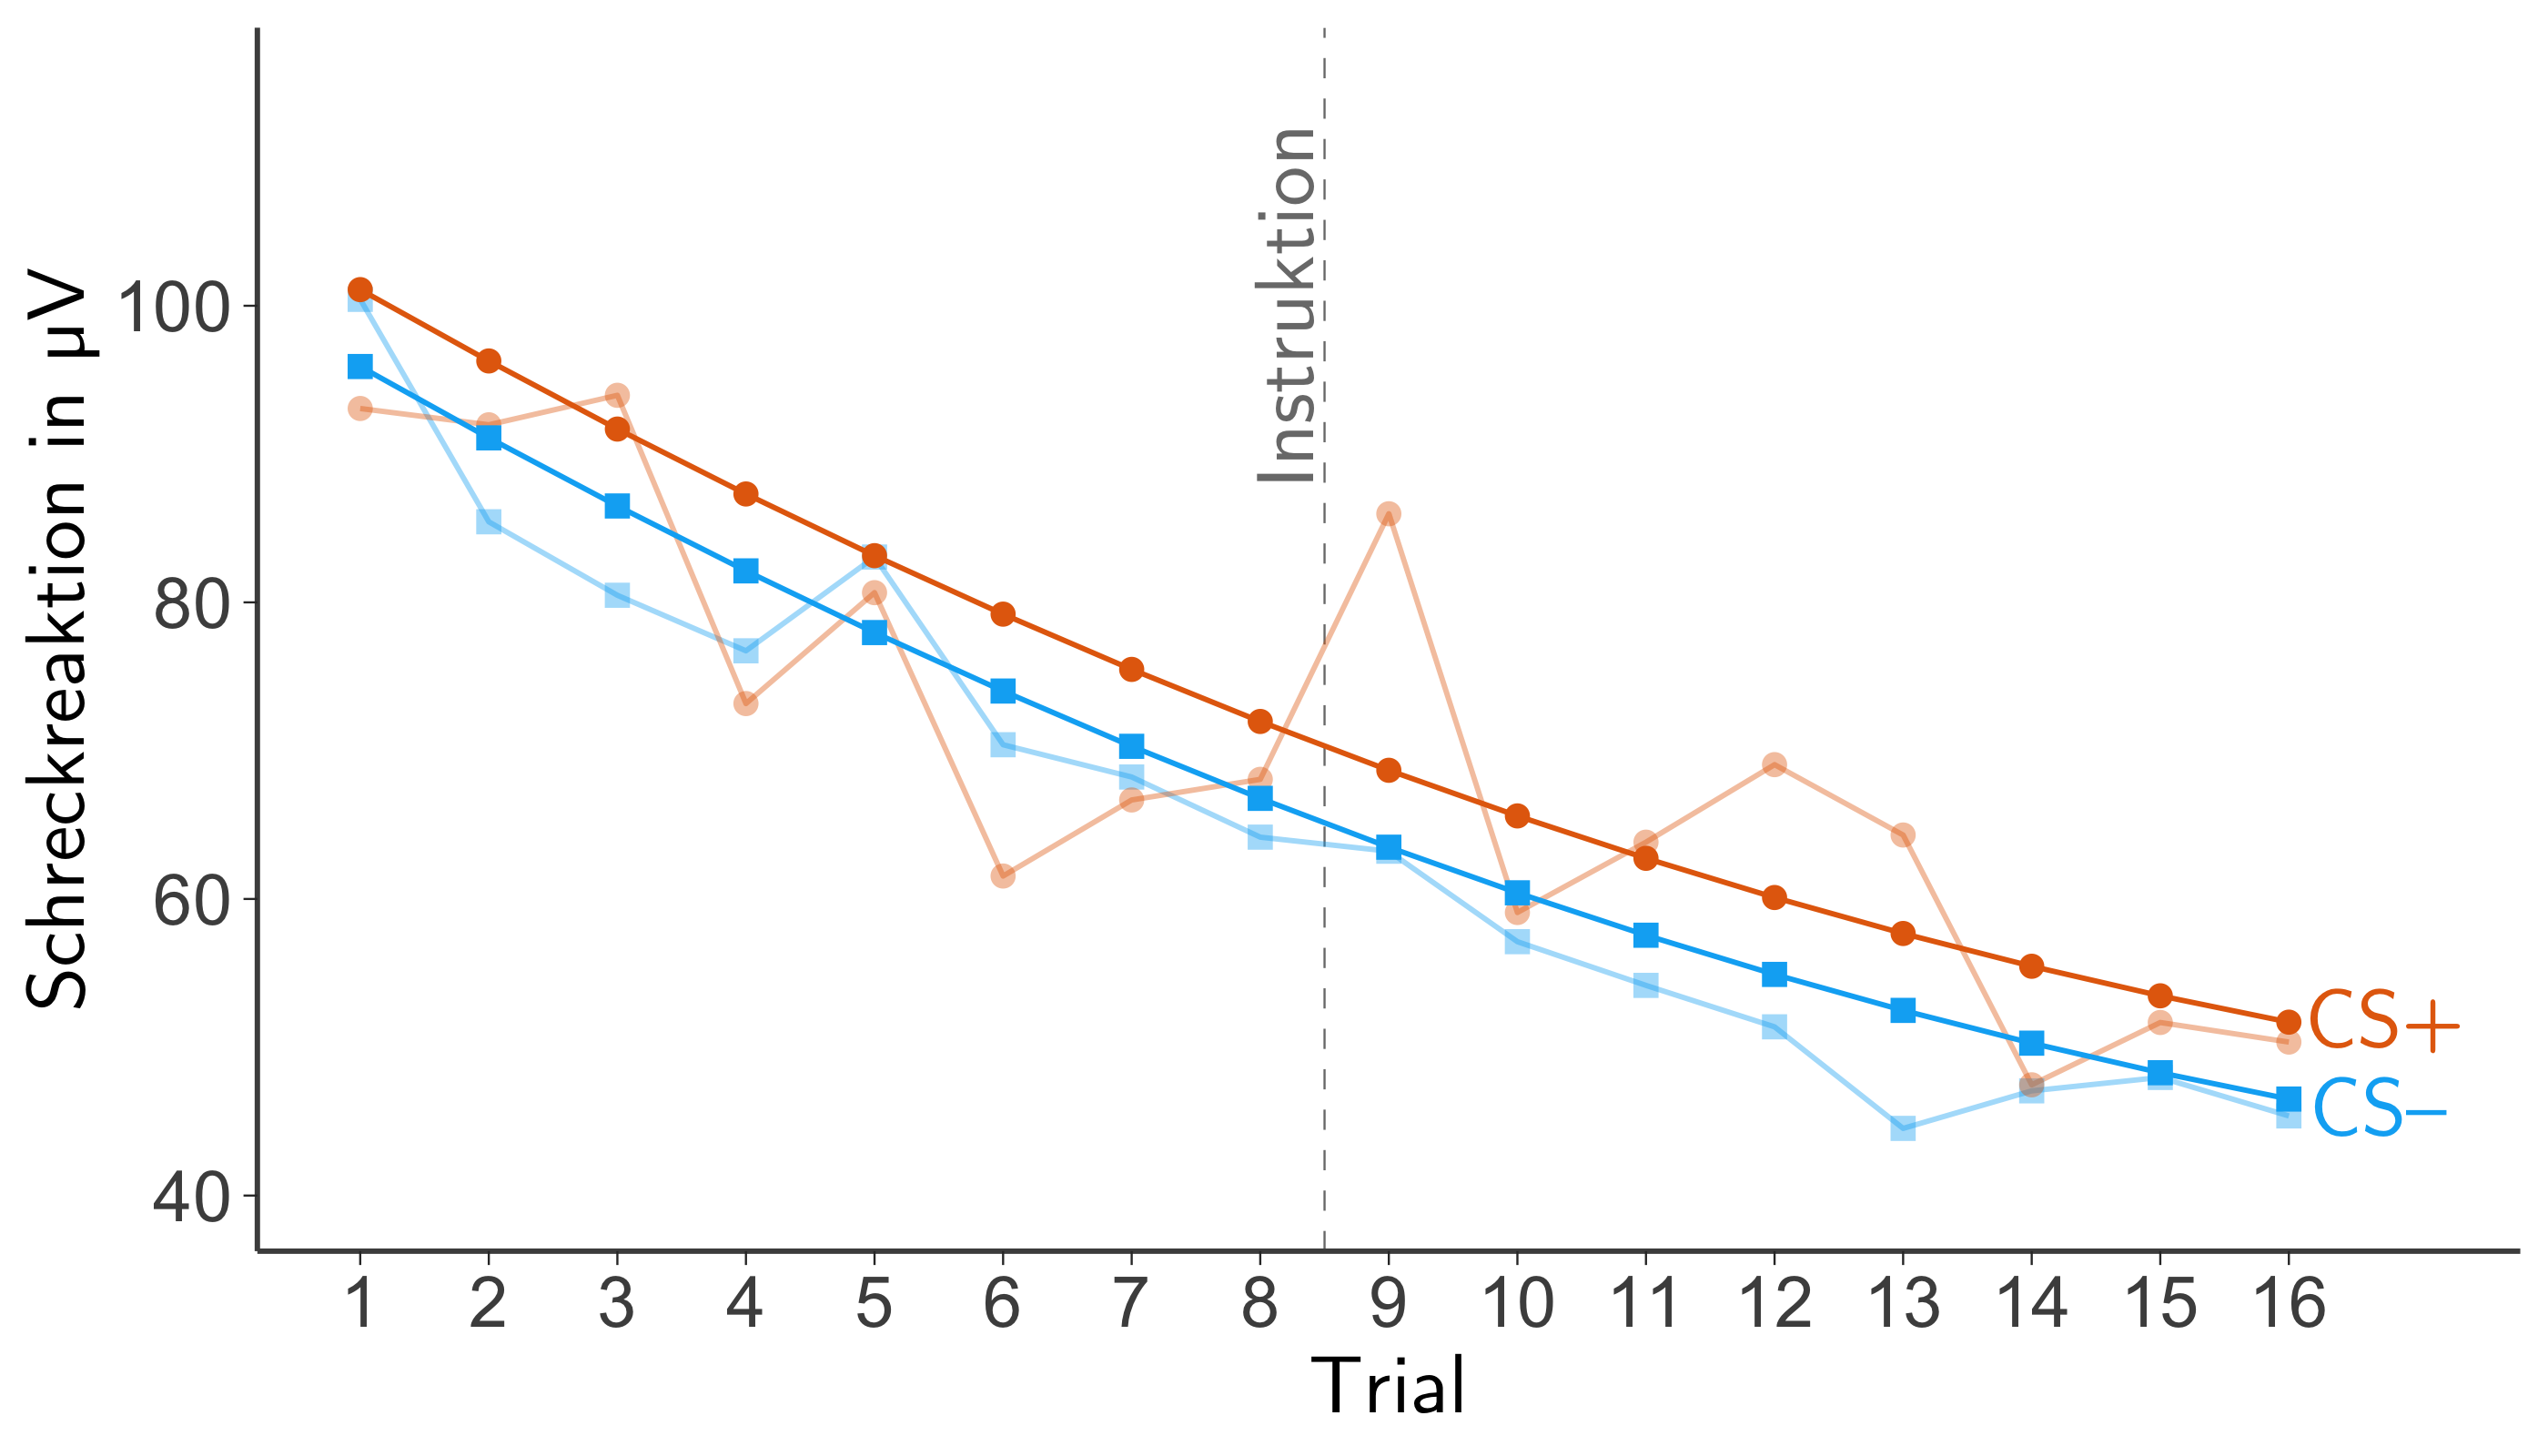
\includegraphics[scale=0.10]{fit_str.png}};
				\node[above left = 0.2cm of scr] (a) {\large{\textsf{\textbf{a}}}};
				\node[above left = 0.2cm of str] (b) {\large{\textsf{\textbf{b}}}};
			\end{tikzpicture}
			\caption[Vorhergesagte Verläufe von Hautleitwert- und Schreckreaktionen]{Vorhergesagte Verläufe von Hautleitwert- (\textsf{\textbf{a}}) und Schreckreaktionen (\textsf{\textbf{b}}) auf Basis des multivariaten Wachstumsmodells, verblasst sind die Rohverläufe.}
			\label{fig:predict}
		\end{figure}
		Im Mittel unterscheidet sich die lineare Änderungsrate für den CS+ also um \SI{0.009}{\micro\siemens} gegenüber der des CS--. Abbildung \ref{fig:predict} zeigt die geschätzten Verläufe nach Stimulustyp getrennt. Hier wird ersichtlich, dass der Unterschied durch einen allmählichen Abfall der Reaktionen auf den CS-- bei relativ gleichbleibender CS+ Reaktion zustande kommt.
		Der beschriebene Interaktionseffekt variiert ebenfalls zwischen Versuchspersonen ($SD=0.006$).
		Die Abweichung der Interaktionsschätzungen für die Versuchspersonen vom festen Effekt $\upbeta_{40}{}^{(1)}$ in Abbildung \ref{fig:randomeffects}e (zentriert bei null) zeigen keine eindeutige Tendenz in Relation zu den zufälligen Intercepts.
		Wenn auch nicht signifikant, deutet allerdings die geschätzte Korrelation zwischen Intercept und Interaktion ($r=-.35$) darauf hin, dass ein höherer Intercept tendenziell mit einem kleineren Unterschied in dem linearen Anstieg zwischen CS+ und CS-- einhergeht.
		
		\begin{table}[hbt] \small \setstretch{1.5} %\doublespacing
			\begin{threeparttable}
				\caption{Ergebnisse des finalen multivariaten Wachstumsmodells}			%ohne Punkt
				\label{tab:final}
				\begin{tabularx}{\textwidth}{lCCCCr}    \toprule
					& \multicolumn{5}{c}{\textbf{Feste Effekte}} \\\cmidrule{2-6} 
					& Beta   & \textit{SE}& \SI{95}{\percent} $KI$		 & $t$   & $p$  \\\hline
					\textbf{SCR} 	 &        &            &                      		       &      &      \\\rowcolor[HTML]{EFEFEF}
					$\quad$Intercept & $0.065$  & $0.029$      &$\left[-0.0008; 0.121\right]$& $2.24$ & $.025$ \\
					$\quad$lin		 & $\hspace*{-0.85em}-0.018$ & $0.004$      &$\left[-0.027; -0.010\right]$& $\hspace*{-0.85em}-4.35$& $<.001$ \\\rowcolor[HTML]{EFEFEF}
					$\quad$CS		 & $0.058$  & $0.012$      &$\left[0.034; 0.083\right]$	 & $4.72$ & $<.001$ \\
					$\quad$CS$\times$lin & $0.009$  & $0.003$      &$\left[0.003; 0.014\right]$	 & $3.00$ & $.003$ \\[+0.5em]	
					\textbf{STR}     &        &            &                      &            &      \\\rowcolor[HTML]{EFEFEF}
					$\quad$Intercept & $\hspace*{-0.5em}59.92$ & $8.49$      &$\left[43.28; 76.57\right]$& $7.06$ & $<.001$ \\
					$\quad$lin		 & $\hspace*{-0.85em}-3.30$ & $0.35$      &$\left[-3.98;-2.60\right]$& $\hspace*{-0.85em}-9.37$& $<.001$ \\\rowcolor[HTML]{EFEFEF}
					$\quad$quad		 & $0.11$  & $0.05$      &$\left[0.01; 0.21\right]$	 & $2.20$ & $.028$ \\
					$\quad$CS 		 & $5.19$  & $1.87$      &$\left[1.53; 8.85\right]$	 & $2.78$ & $.006$ \\
					%&&&&&\\[-0.2em]\bottomrule
				\end{tabularx}
				\begin{tabularx}{\textwidth}{lCccccc}    \toprule
					& \multicolumn{6}{c}{\textbf{Zufällige Effekte}}\\ \cmidrule{2-7} 
					& \multirow[c]{2}{*}{\textit{SD}} & \multirow[c]{2}{*}{\SI{95}{\percent} $KI$} && \multicolumn{3}{c}{Korrelationen\tnote{a}}    \\ 
					&&       && Intercept (SCR) & Intercept (STR)& CS$\times$lin (SCR)      \\ \hline \rowcolor[HTML]{EFEFEF}
					Intercept (SCR) 		 & $0.130$ &$\left[0.10;0.17\right]$&& --           	  &      		 &      	\\
					Intercept (STR) 		 & $\hspace*{-0.5em}49.98$&$\left[39.8;62.7\right]$&& $.14$	          & --     		 &       \\\rowcolor[HTML]{EFEFEF}
					CS$\times$lin (SCR) 	 & $0.006$ &$\left[0.004;0.009 \right]$&& $\hspace*{-0.85em}-.35$          & $-.04$ 		 & --    \\
					CS$\times$lin (STR) 	 & $1.341$ &$\left[0.99;1.81\right]$&& $\hspace*{-0.85em}-.05$          & $\hspace*{0.55em}-.48^*$ 		 & $-.29$ \\[-0.2em]
					\bottomrule
				\end{tabularx}
				\begin{tablenotes}[normal, flushleft, para]
					\footnotesize{
						\item \textit{Anmerkungen.} Konfidenzintervalle, Signifikanz und $p$-Werte berechnet über Normalapproximationen der Verteilung der geschätzten Effekte. Die daraus angenäherte $t$-Teststatistik hat $df=2374$ Nenner-Freiheitsgrade.
						\item[a] bei ${}^{*}$ signifikant auf \SI{5}{\percent} Niveau.}
				\end{tablenotes}
			\end{threeparttable}
		\end{table}	
		
		Für die Schreckreaktion beschreibt der geschätzte Intercept mit \SI{59.92}{\micro\volt} ebenfalls die mittlere Reaktion zwischen dem $8.$ und $9.$ CS-- Trial ($SE=8.49$). Als zufällig modelliert variiert dieser Intercept mit einer geschätzten Standardabweichung von $49.98$ zwischen Versuchspersonen. Abbildungen \ref{fig:randomeffects}b und \ref{fig:randomeffects}d zeigen die Versuchspersonen-Intercepts als Abweichungen vom mittleren Intercept. Hier liegen die geschätzten Intercept nur für zwei knapp unter Null.
		Der Koeffizient $\upbeta_{10}{}{(2)}$ mit der Schätzung $-3.3$ ($SE=0.35$) reflektiert nun die momentane Änderungsrate der Schreckreaktion für den CS-- in der Mitte des Akquisitionstrainings. Die quadratische Änderungsrate für den CS-- ist positiv ($\upbeta_{20}{}{(2)}=0.11$, $SE=0.05$). Daraus und in Verbindung mit Abbildung \ref{fig:predict} wird deutlich, dass die Wachstumskurven für die Schreckreaktion als nach oben geöffnete, gestauchte Parabeln modelliert werden. 
		Auch hier hat der Stimulustyp einen substanziellen Einfluss. Im Mittel sind die Schreckreaktionen der Versuchspersonen auf den CS+ \SI{5.19}{\micro\volt} höher als auf den CS-- ($SE=1.87$). Allerdings ist die Interaktion -- sprich der Unterschied zwischen CS+ und CS-- in der linearen Änderungsrate -- im Gegensatz zur SCR statistisch nicht bedeutsam. Über die Zeit hinweg wird der Unterschied zwischen CS+ und CS-- daher als konstant modelliert (Abb. \ref{fig:predict}).
		Die Varianz, die Versuchspersonen in dieser Interaktion aufzeigen, ist wiederum Teil des Modells. Für den zufälligen Effekt zeigt sich, dass die Interaktionseffekte zwischen Versuchspersonen mit einer Standardabweichung von $1.34$ variieren.
		In der Abbildung \ref{fig:randomeffects}f lässt sich durch Hinzunahme der nach Größe geordneten Interceptschätzungen aus \ref{fig:randomeffects}d ein Abwärtstrend vermuten, den die geschätzte Korrelation von $r=-.48$ zwischen Intercept und Interaktion bestätigt. Für Versuchspersonen mit höherer Reaktion auf den CS-- in der Mitte des Trainings werden eher kleinere Unterschiede im linearen Anstieg zwischen CS+ und CS-- vorhergesagt. Der \nameref{appE} enthält unterstützend paarweise Streudiagramme zwischen den geschätzten zufälligen Effekten innerhalb und zwischen den beiden Reaktionsmaßen.
		In der multivariaten Betrachtung zeigt sich ein positiver, kleiner und nicht signifikanter Zusammenhang ($r=.14$). %Ein größerer Mittelwert in der Hautleitwertreaktion auf den CS-- in der Mitte des Trainings geht daher3 tendenziell mit einem größeren Mittelwert der Schreckreaktion einher. 
		Bei den beiden Interaktionseffekten \textit{CS$\times$lin} schätzt das Modell eine negative Korrelation von $r=-.29$ zwischen den abhängigen Variablen, die allerdings wiederum nicht signifikant ist. Tendenziell geht damit ein größerer Interaktionsterm auf dem einen Reaktionsmaß mit einer kleineren Interaktion auf dem anderen Maß einher.
		%Die vorhergesagte mittlere Reaktion auf einen CS+ in der Mitte des Akquisitionstrainings wäre damit $58.12+5.26=63.38$
	
		\begin{figure}[ht]
			\centering
			\begin{tikzpicture}[remember picture] \centering		
				\node[inner sep=0pt] (a1) at (0,0)
				{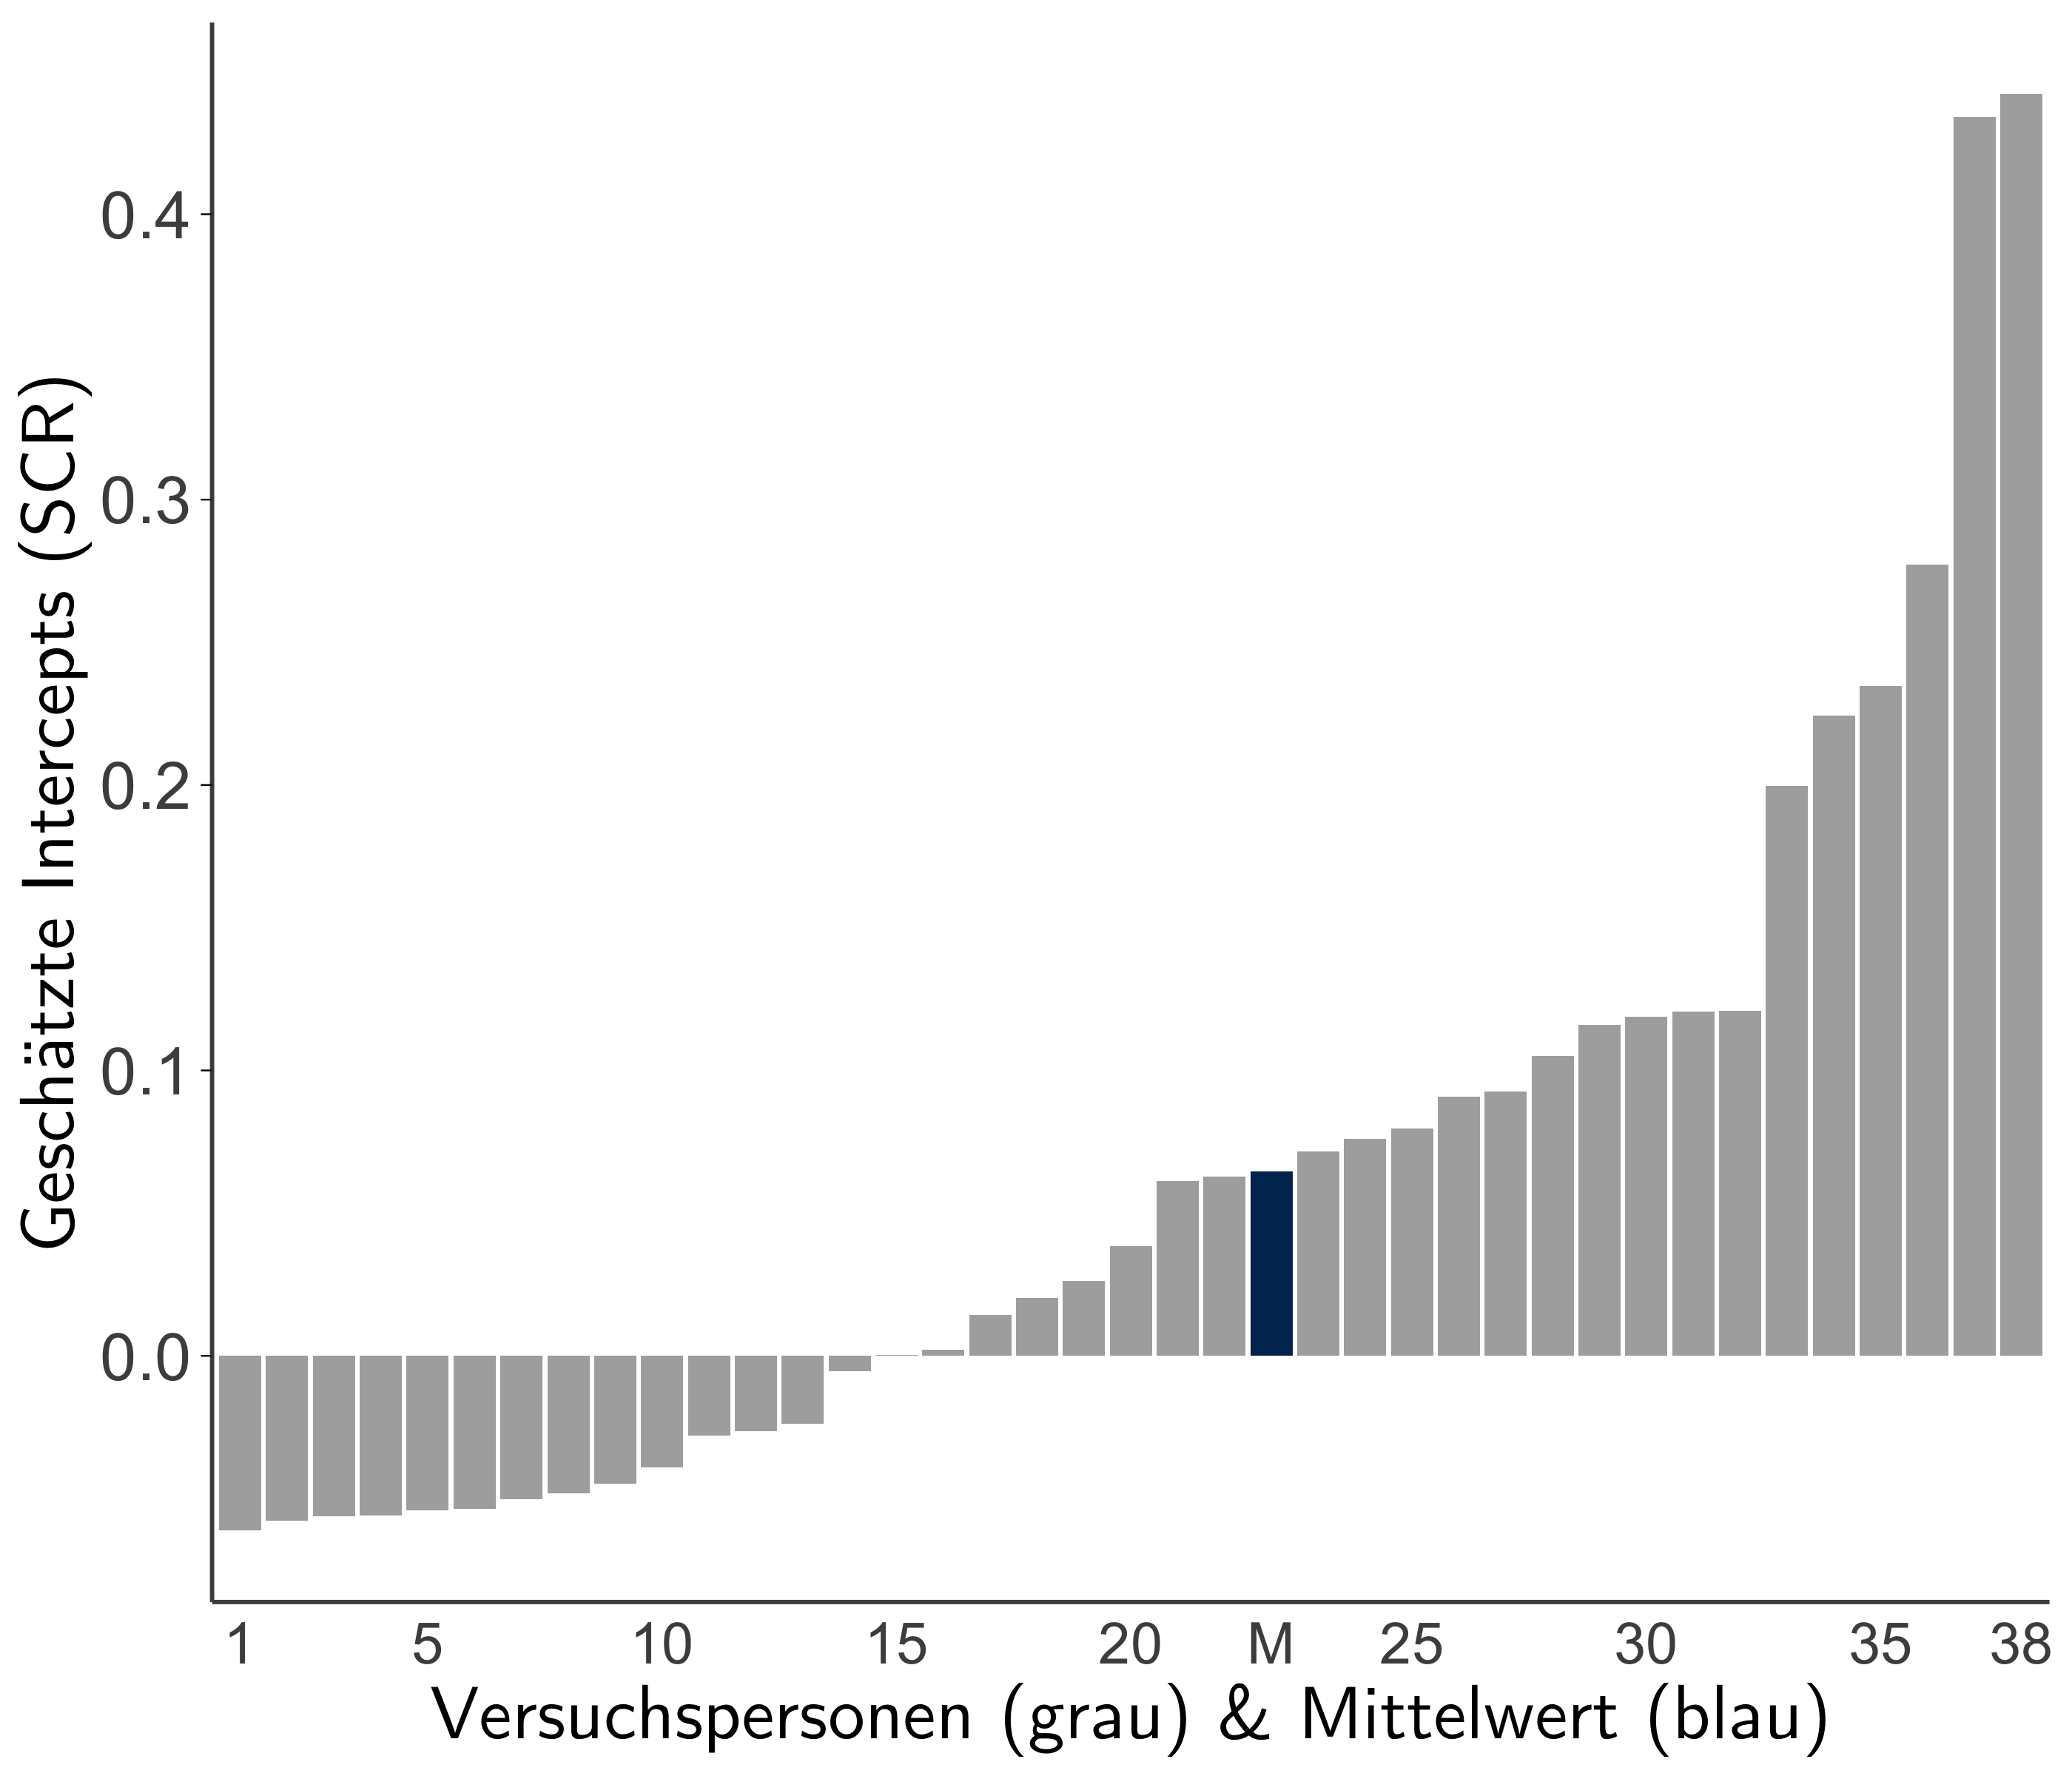
\includegraphics[scale=0.068]{r1.png}};
				\node[inner sep=0pt, below = 0.7cm of a1] (a2)
				{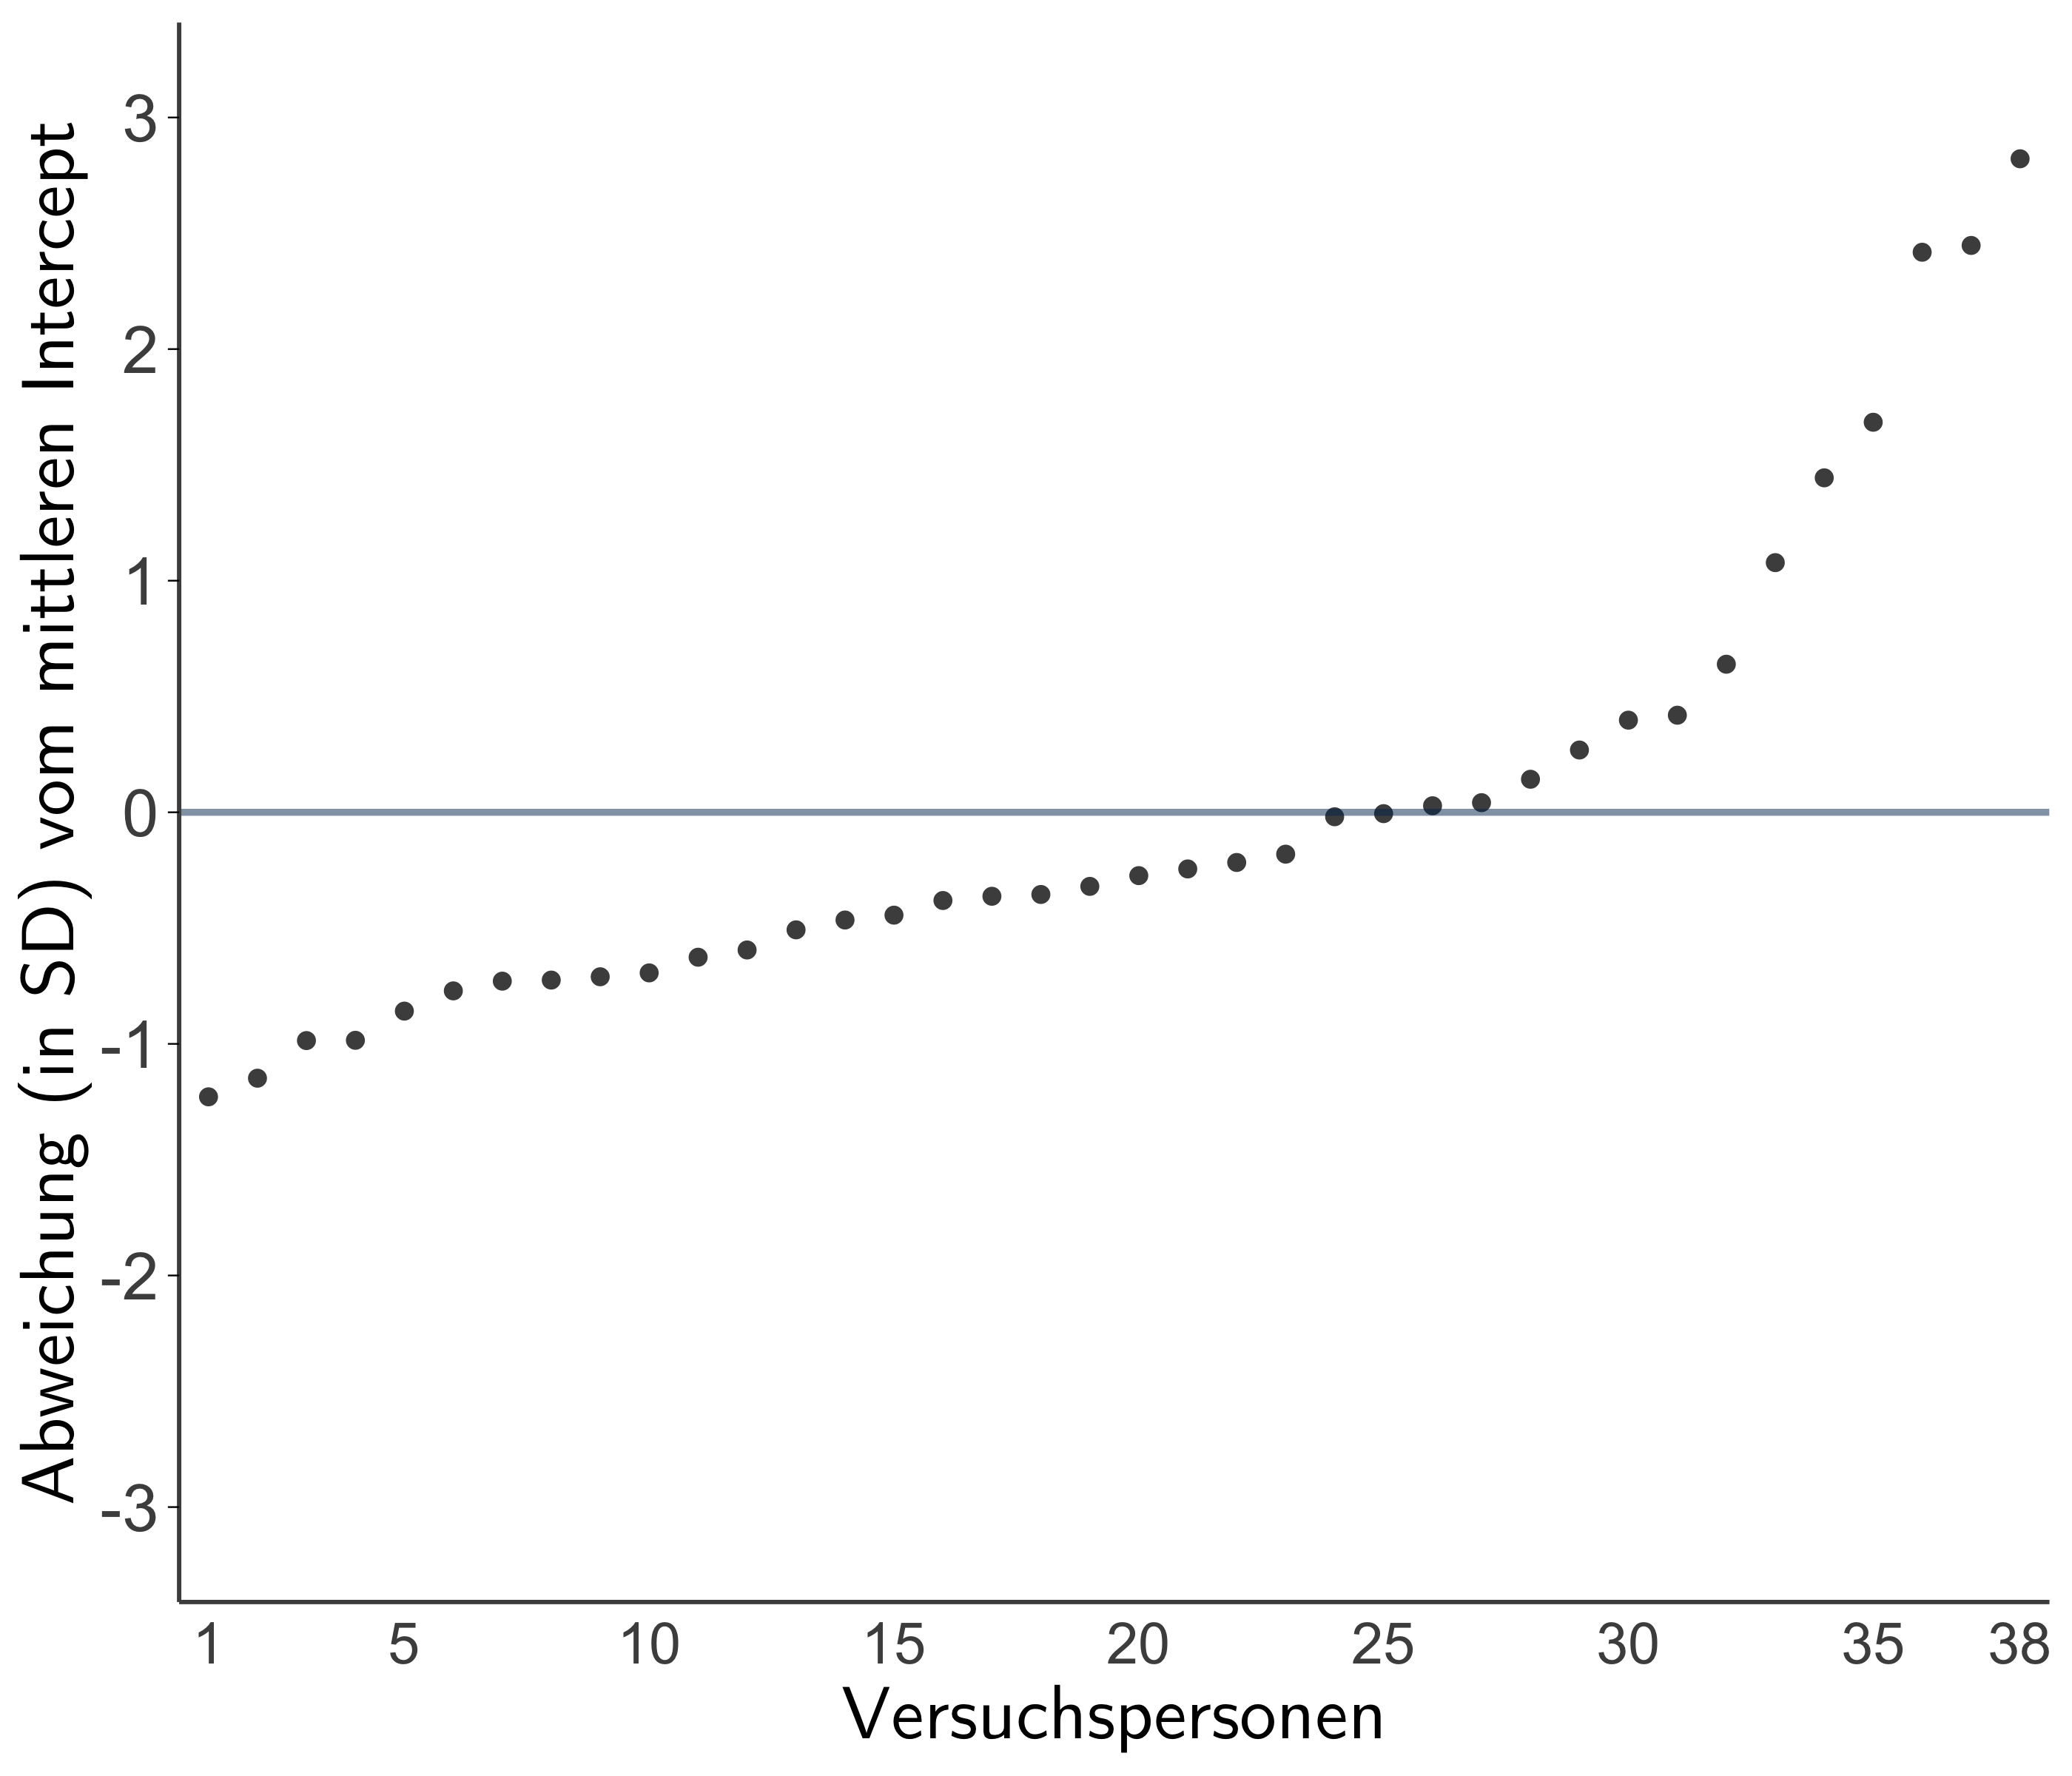
\includegraphics[scale=0.068]{r4.png}};
				\node[inner sep=0pt, right = 1cm of a1] (a3)
				{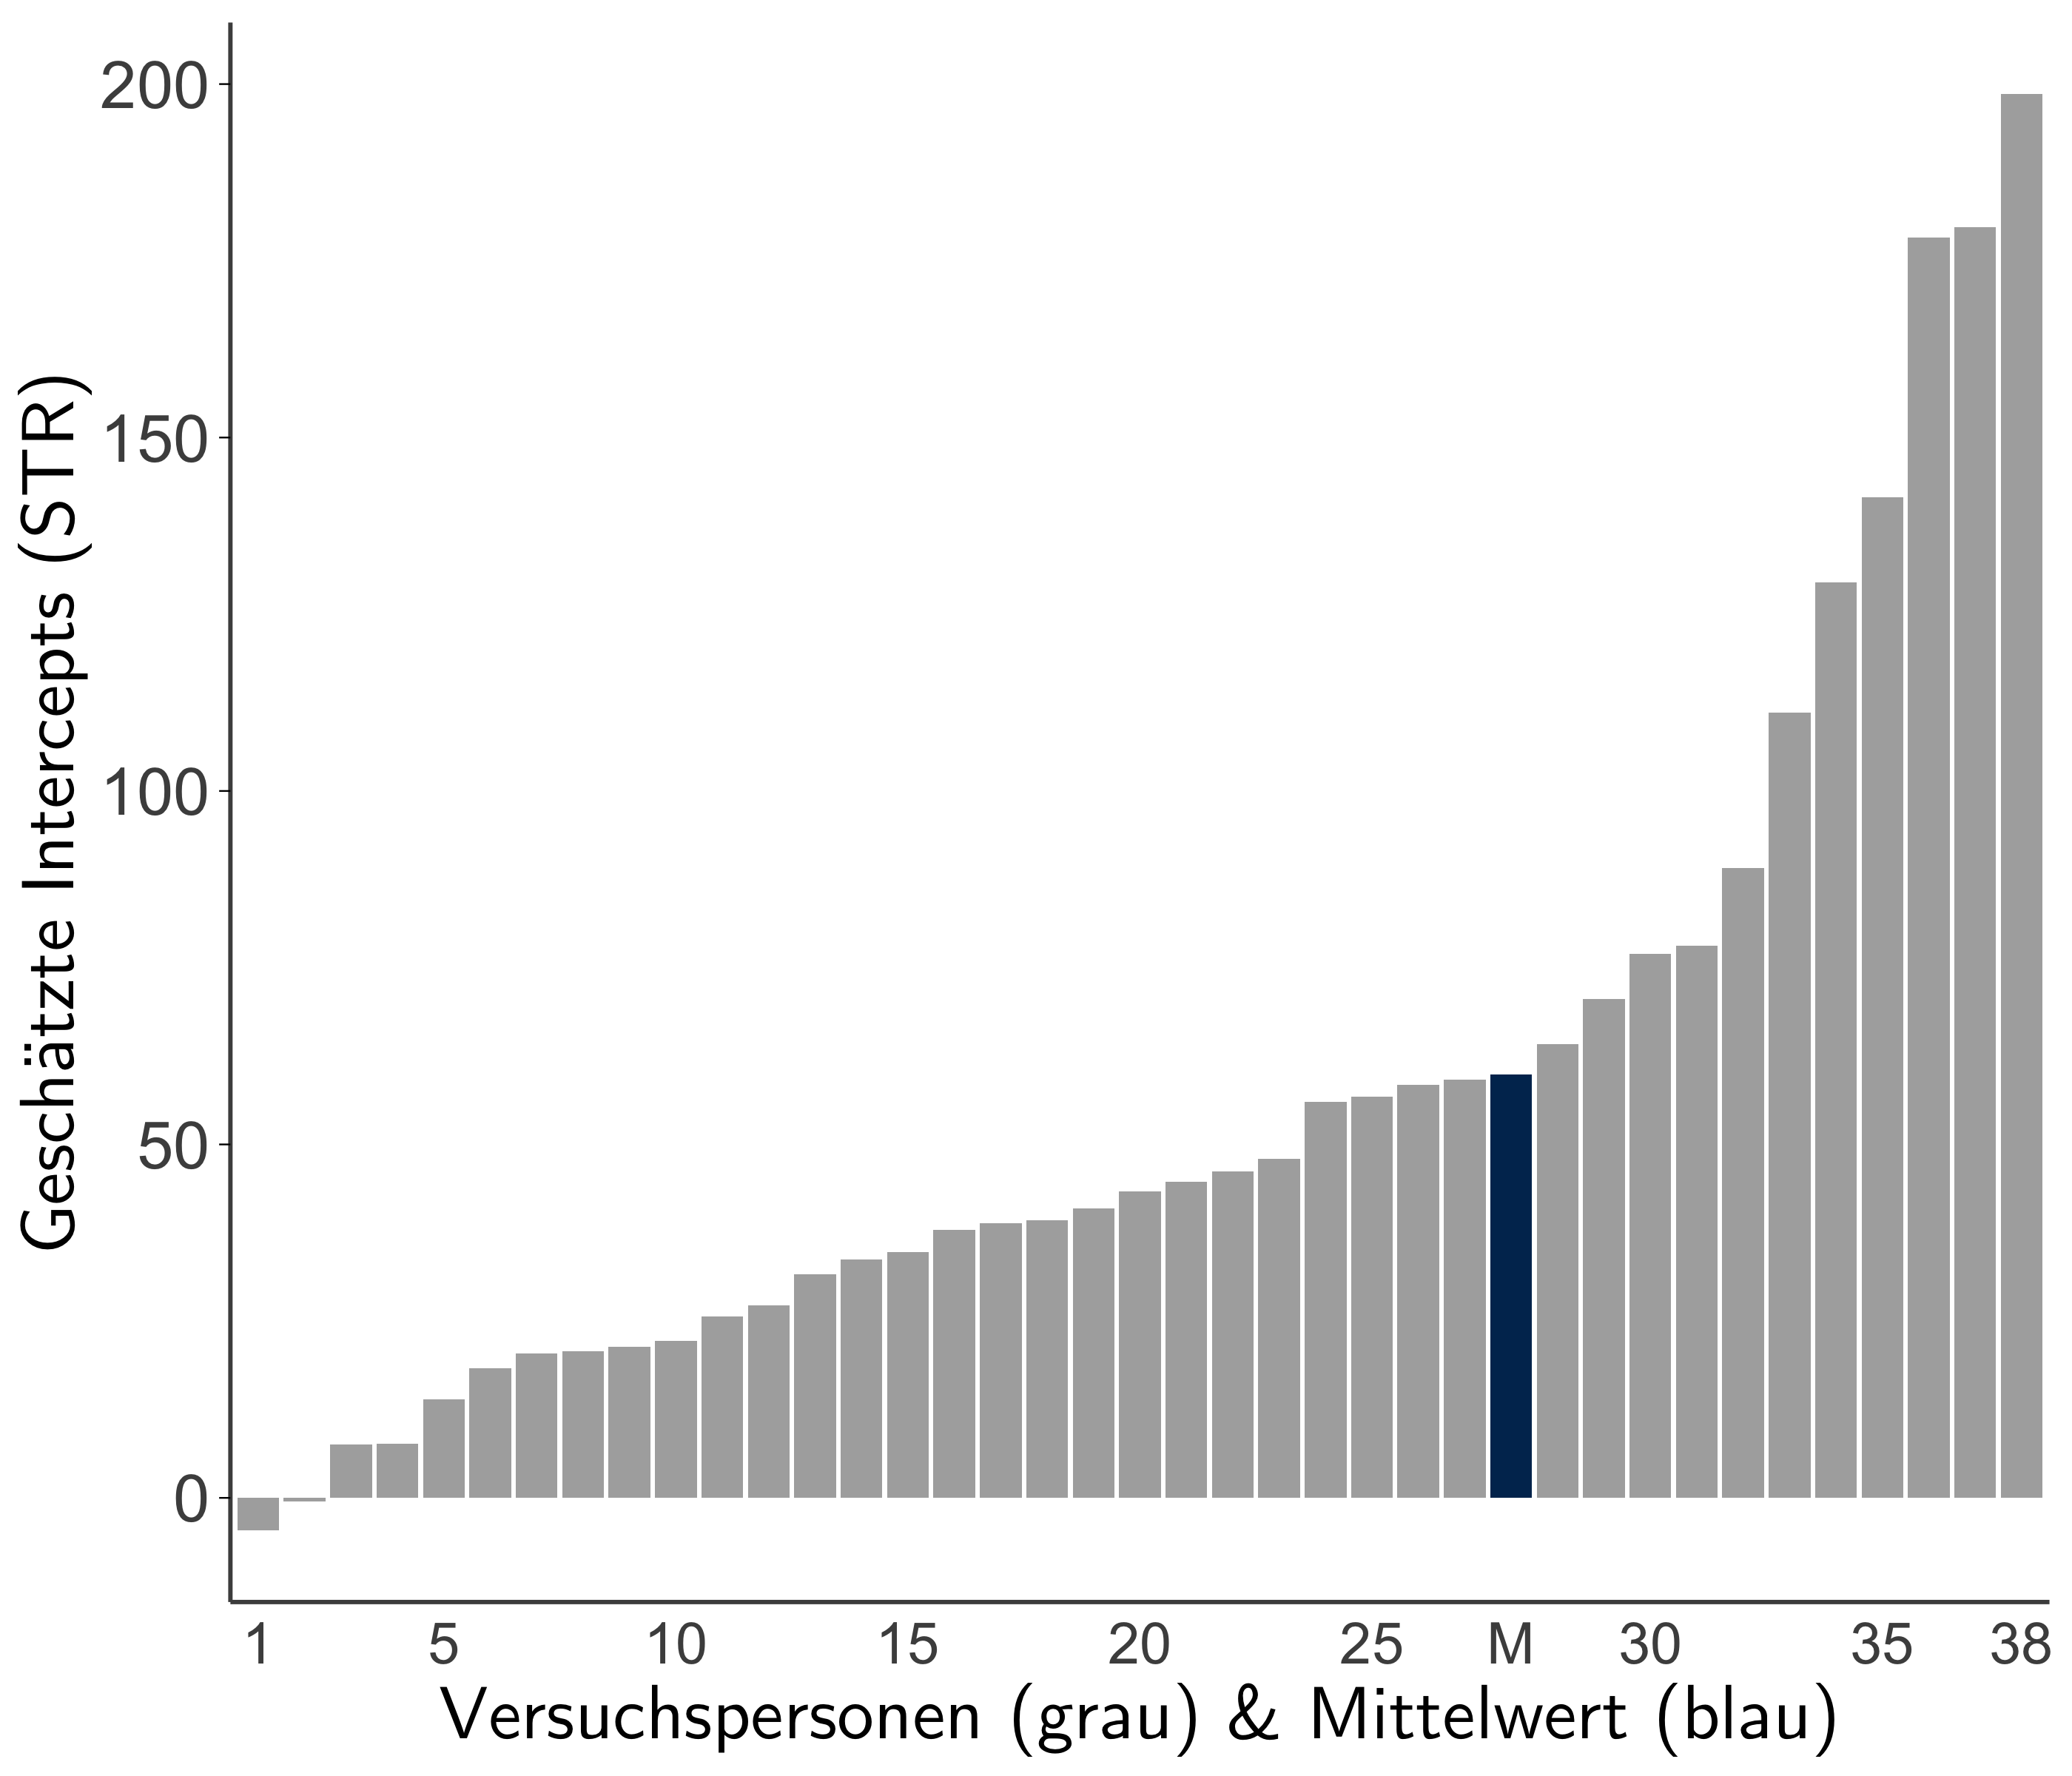
\includegraphics[scale=0.068]{r2.png}};
				\node[inner sep=0pt, below = 0.7cm of a3] (a4)
				{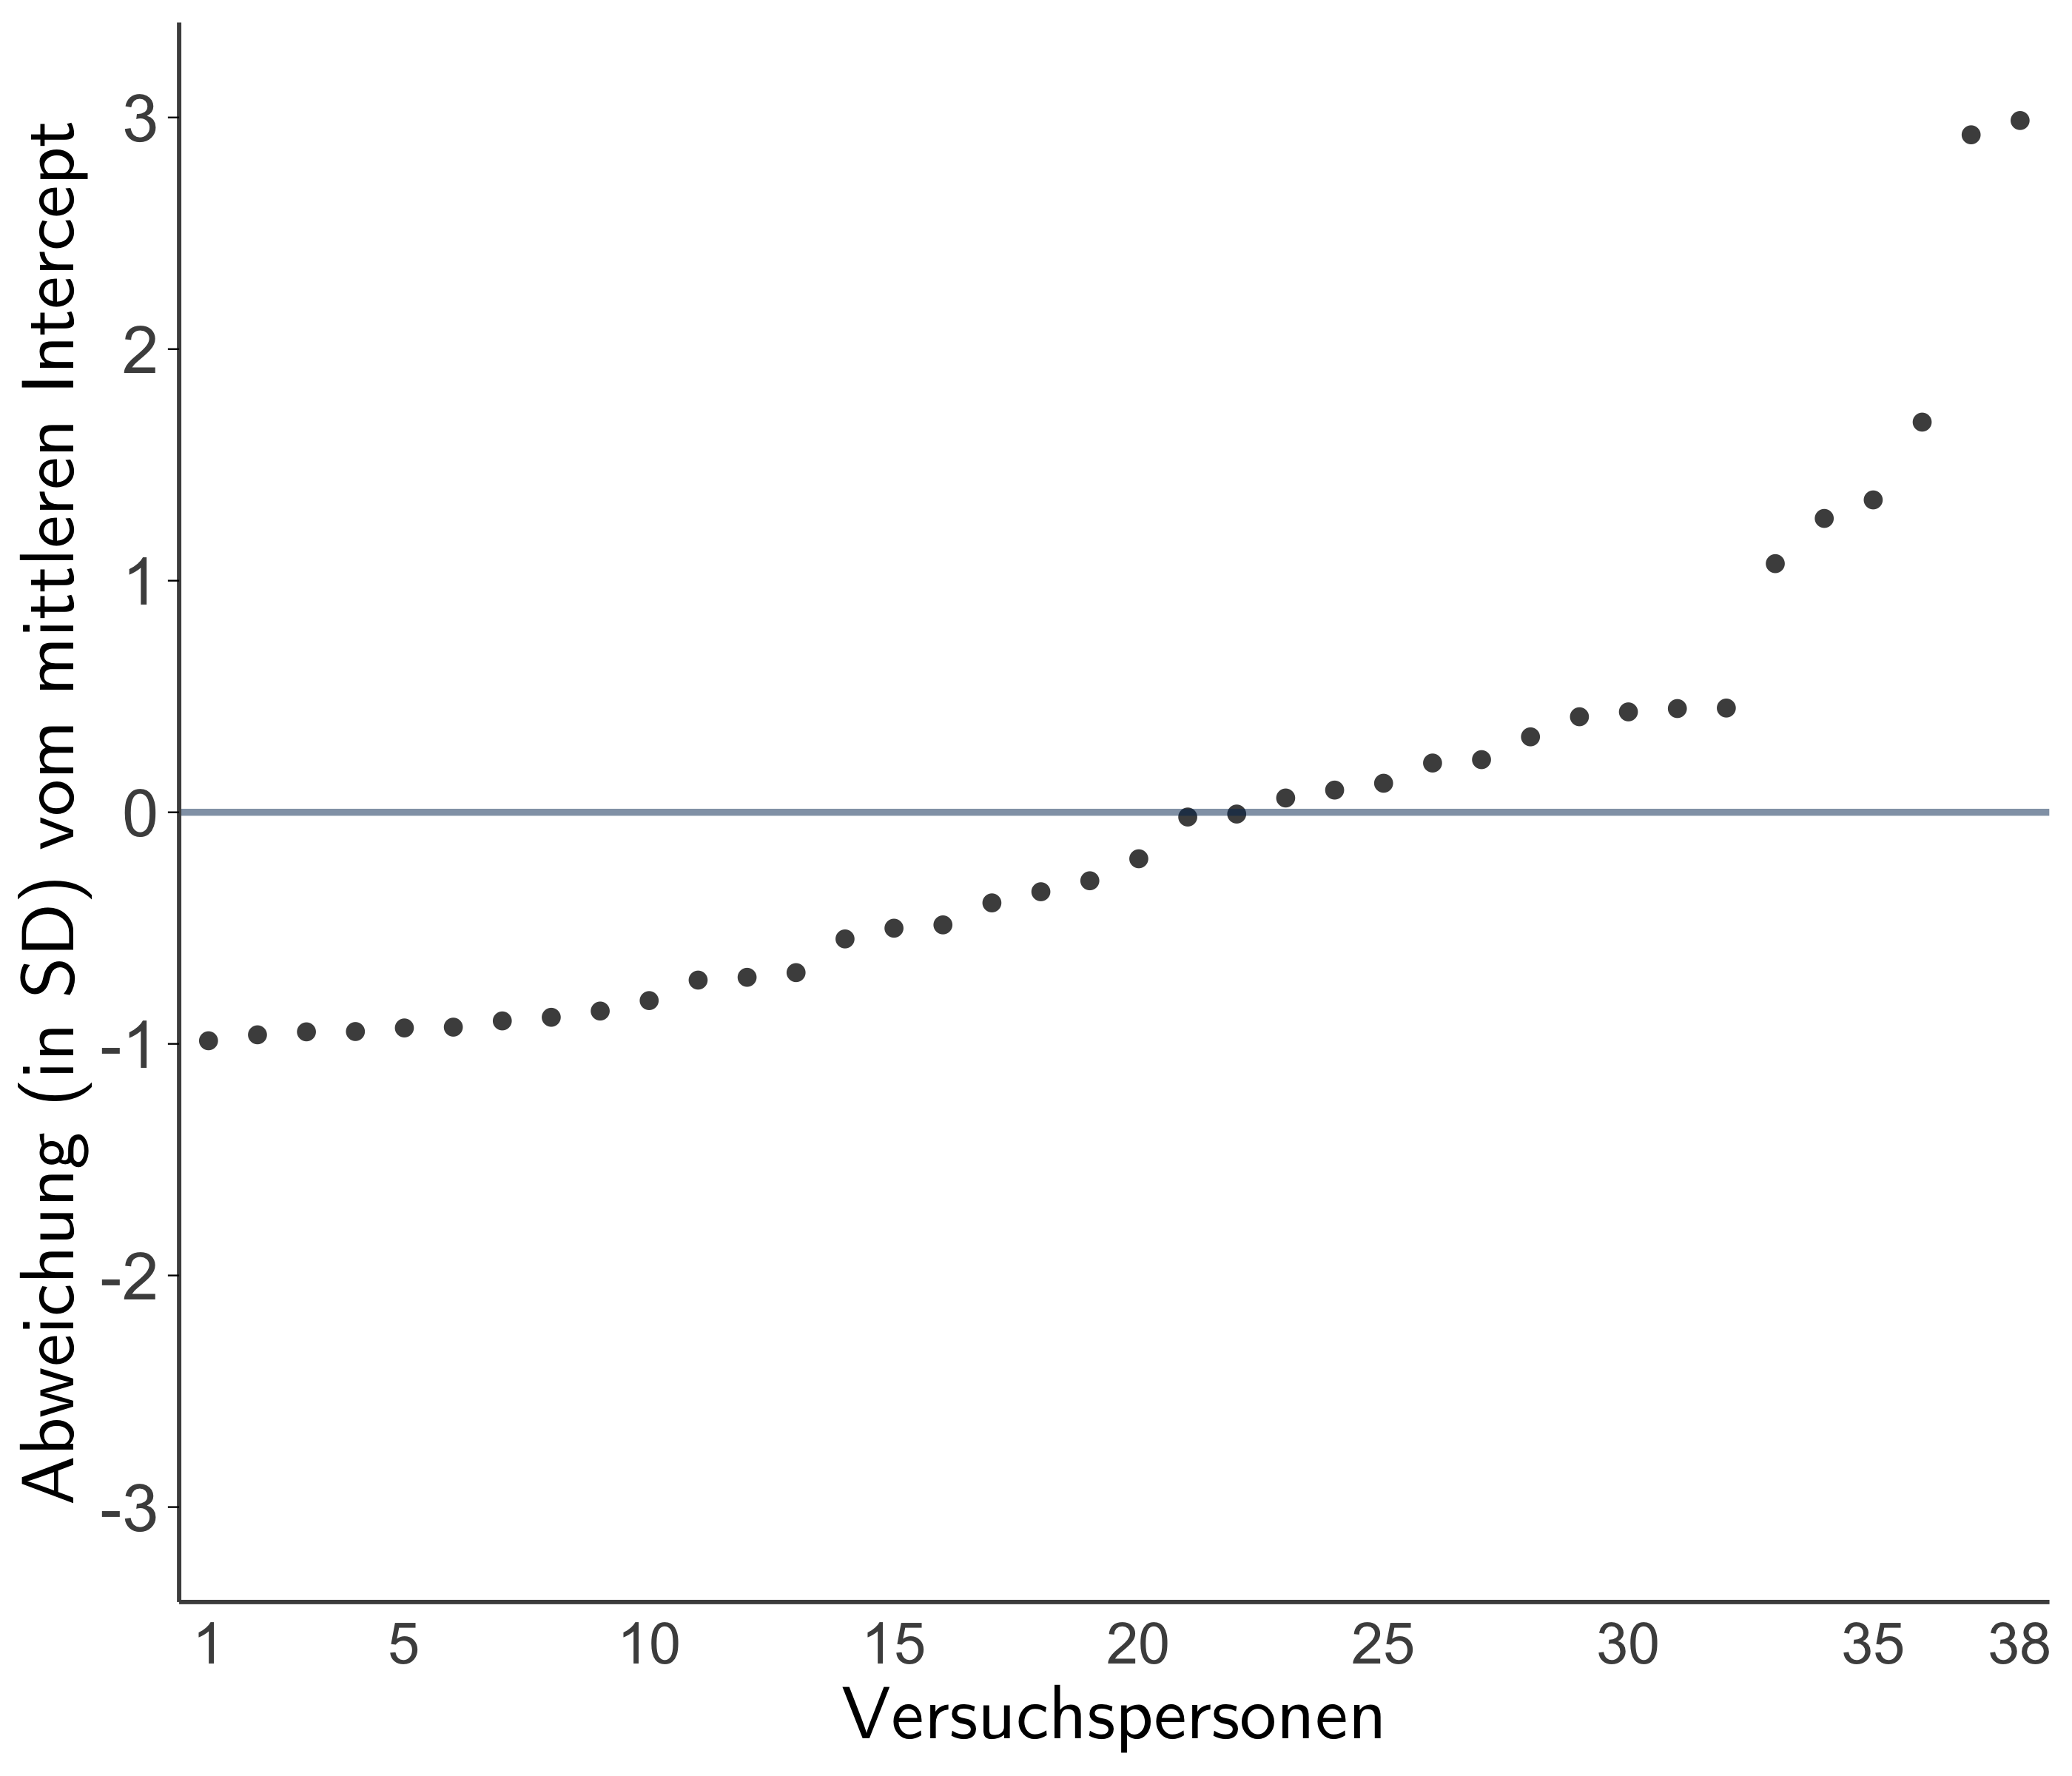
\includegraphics[scale=0.068]{r5.png}};
				\node[inner sep=0pt, below = 0.7cm of a2] (a5)
				{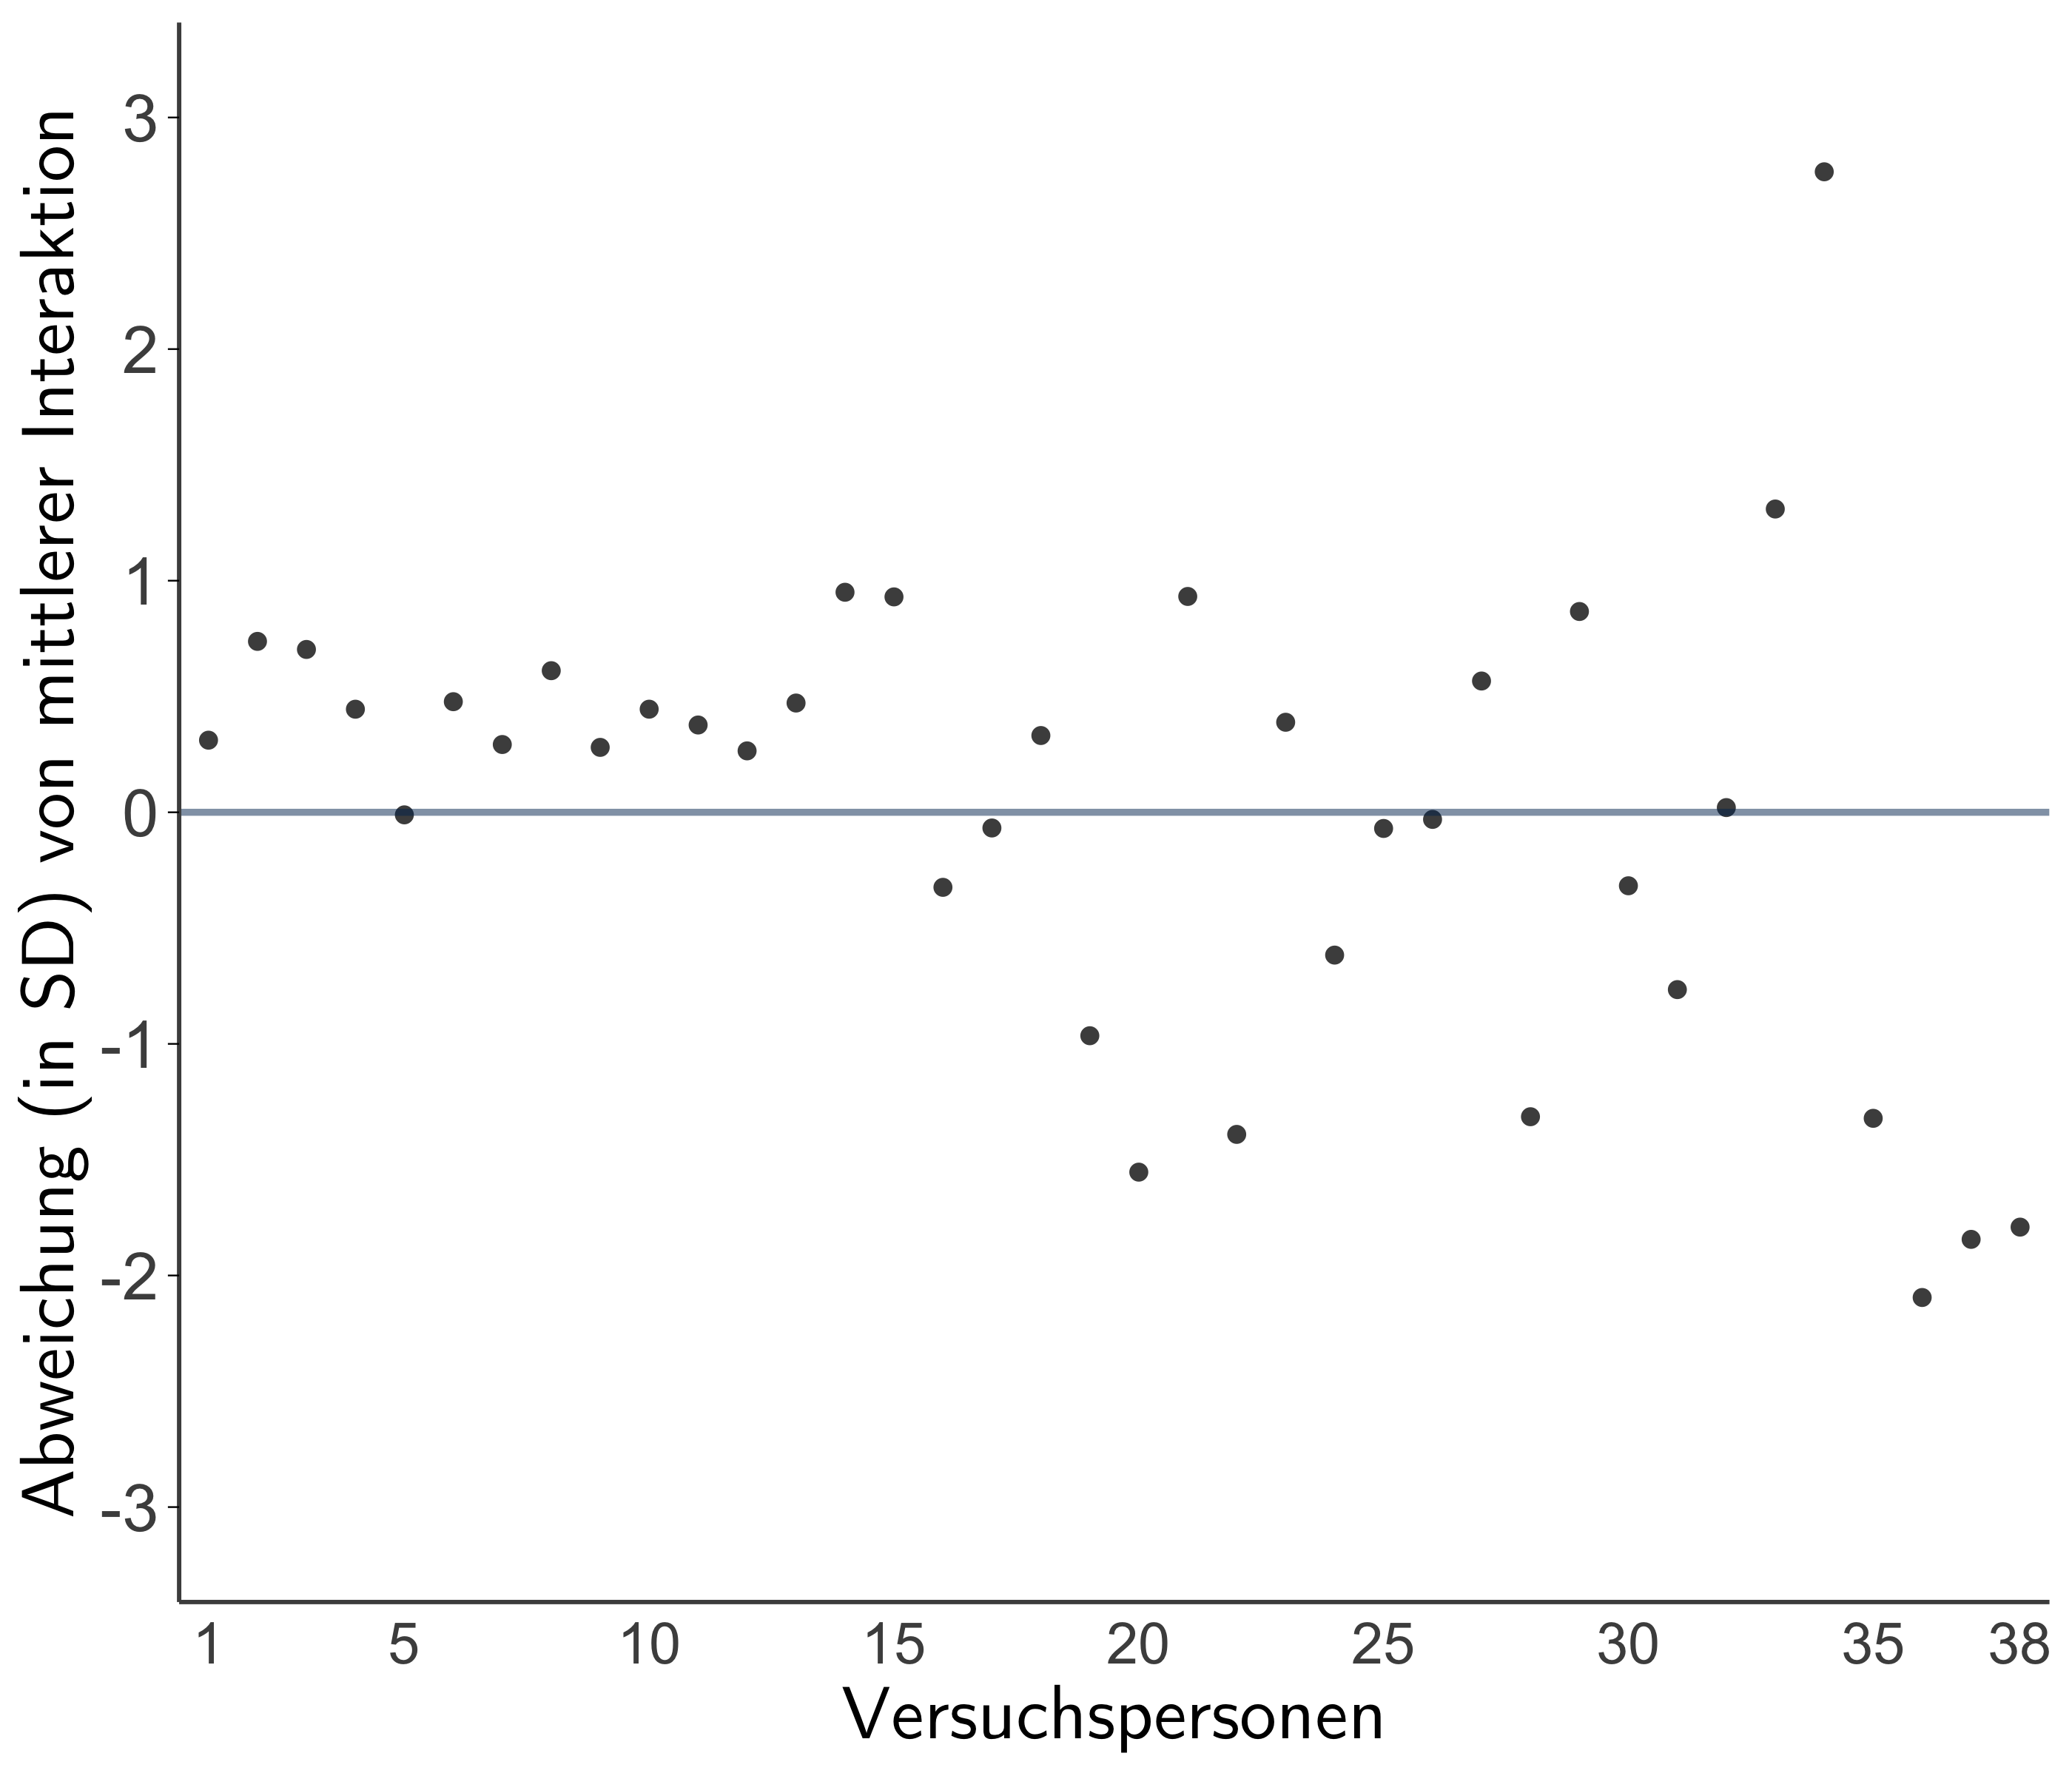
\includegraphics[scale=0.068]{r7.png}};
				\node[inner sep=0pt, right = 1cm of a5] (a6)
				{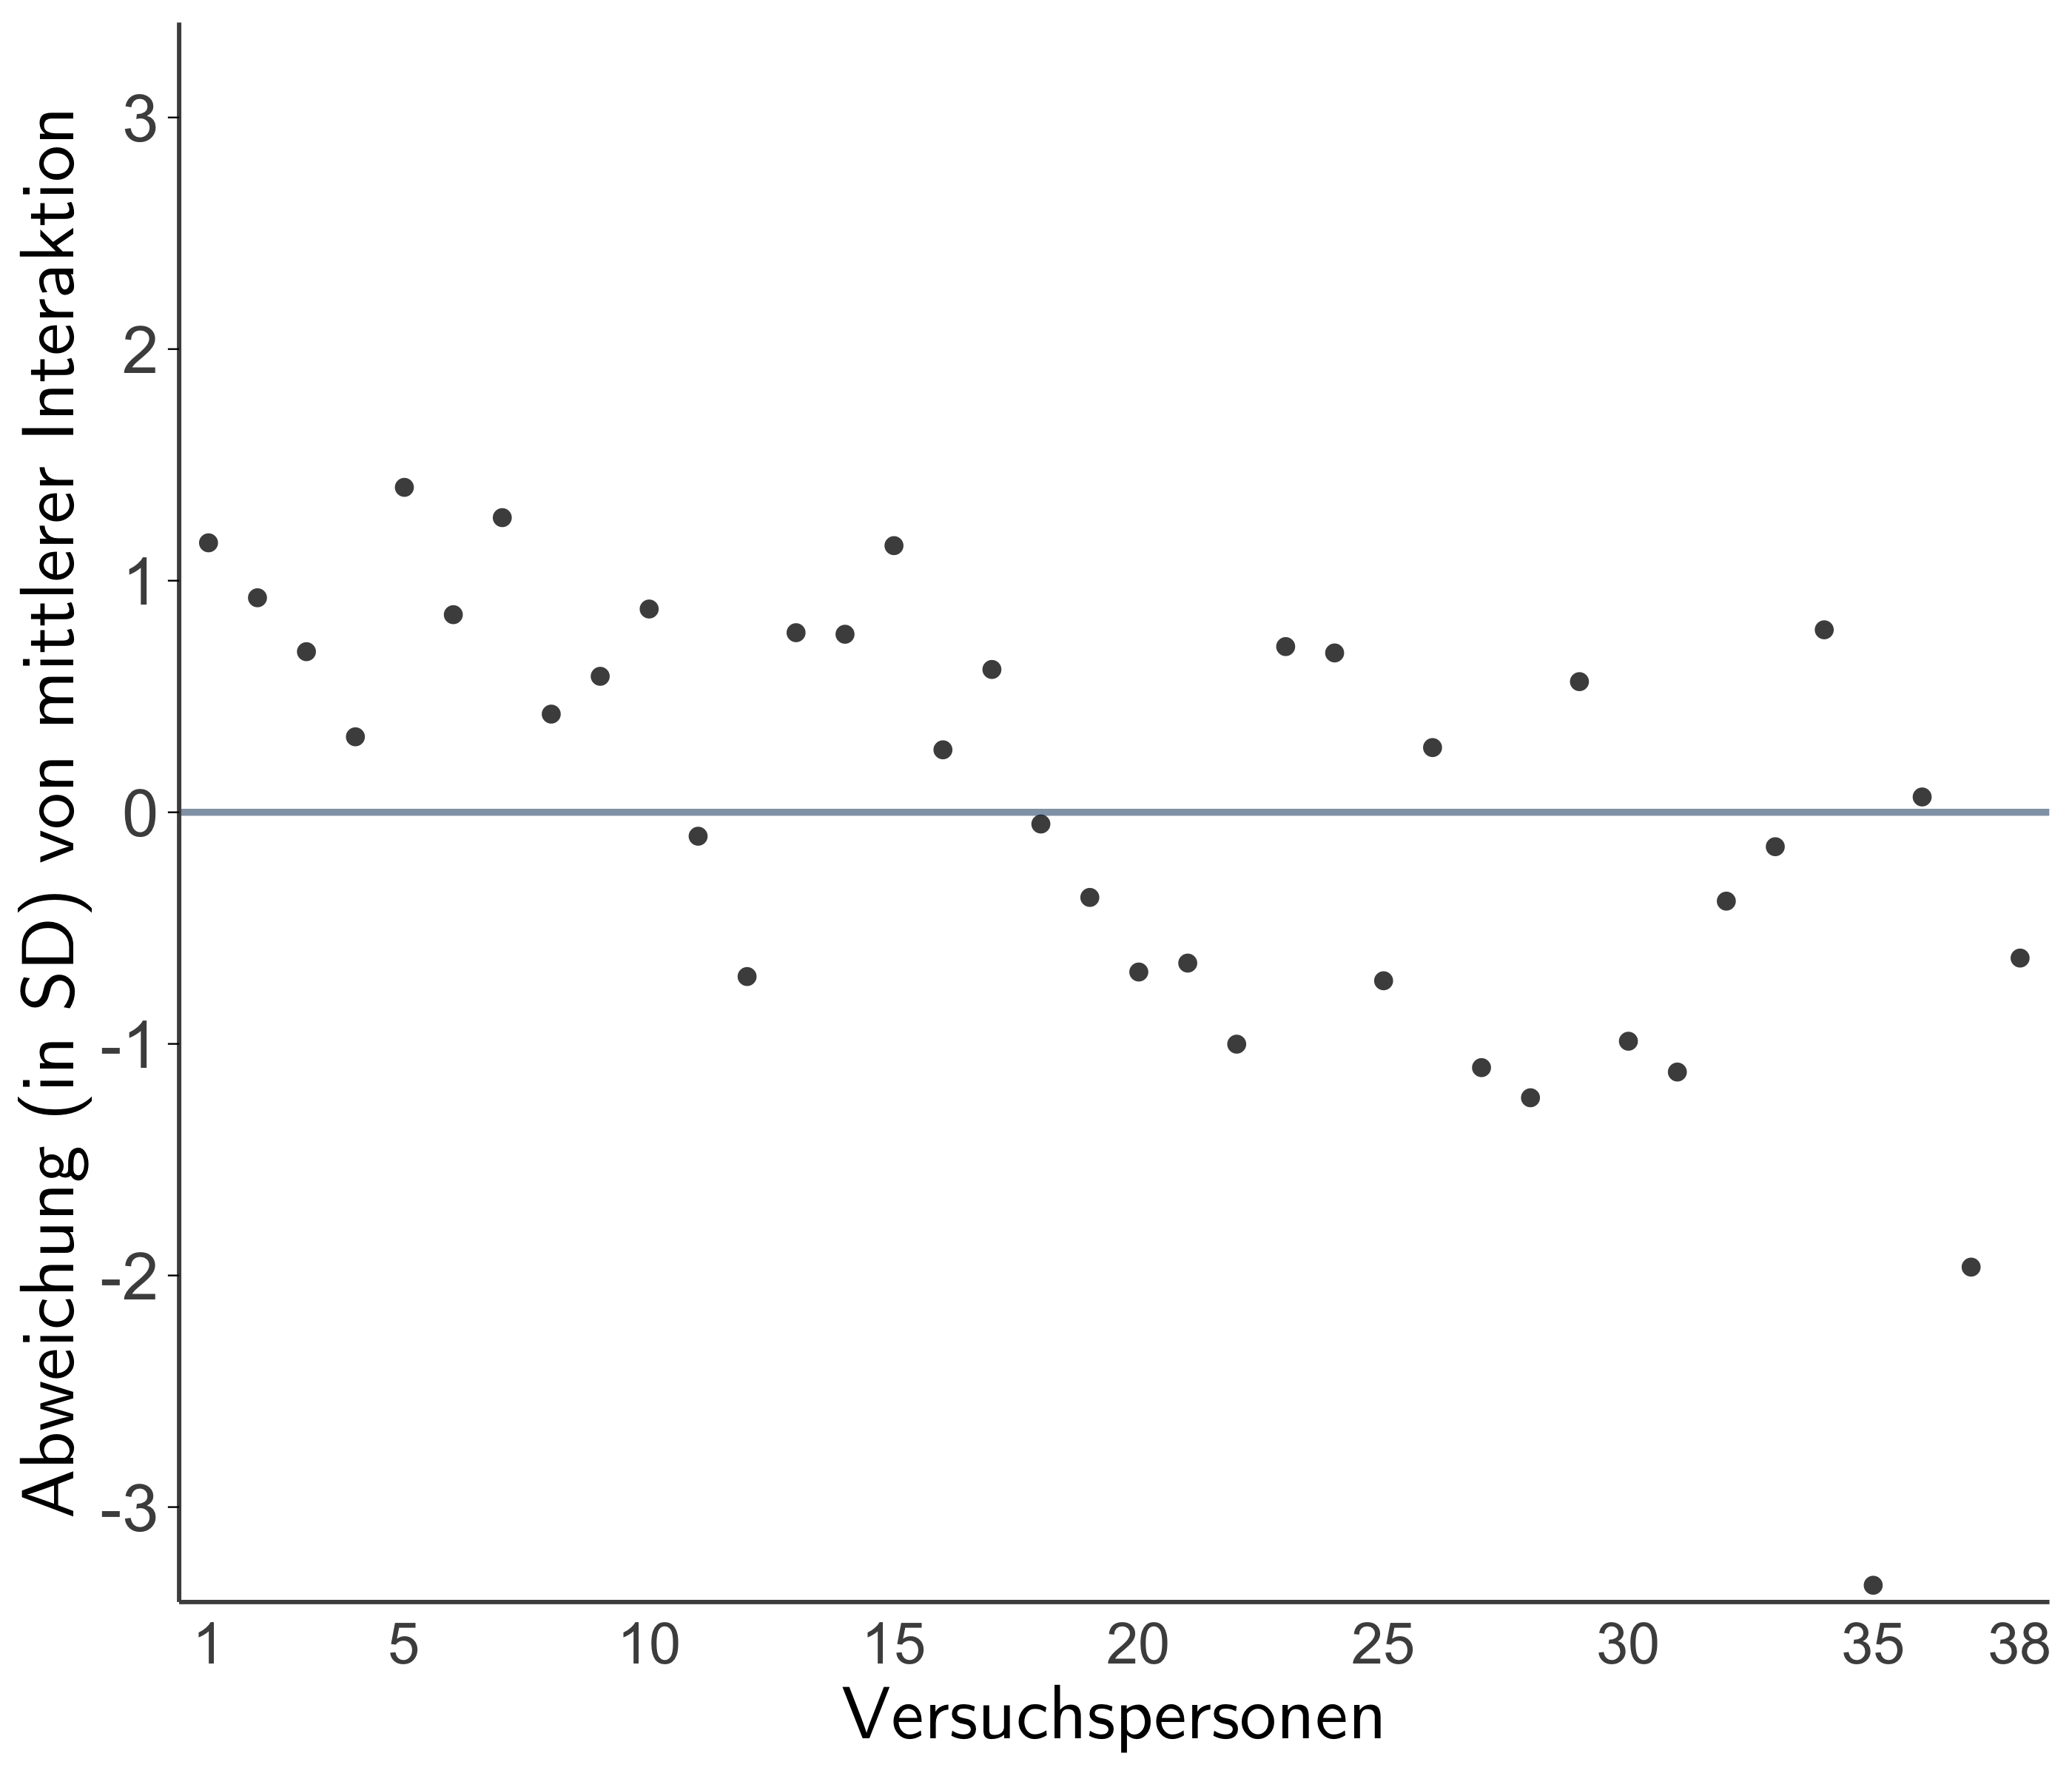
\includegraphics[scale=0.068]{r6.png}};
				\node[above = 0.7cm of a1] (SCR) {\large{\textsf{\textbf{SCR}}}};
				\node[above = 0.7cm of a3] (STR) {\large{\textsf{\textbf{STR}}}};
				\node[above left = 0.1cm and -0.5cm of a1] (a) {\large{\textsf{\textbf{a}}}};
				\node[above left = 0.1cm and -0.5cm of a3] (b) {\large{\textsf{\textbf{b}}}};
				\node[above left = 0.1cm and -0.5cm of a2] (c) {\large{\textsf{\textbf{c}}}};
				\node[above left = 0.1cm and -0.5cm of a4] (d) {\large{\textsf{\textbf{d}}}};
				\node[above left = 0.1cm and -0.5cm of a5] (e) {\large{\textsf{\textbf{e}}}};
				\node[above left = 0.1cm and -0.5cm of a6] (f) {\large{\textsf{\textbf{f}}}};
			\end{tikzpicture}
			\caption[Abbildung der zufälligen Intercepts \& Interaktionen]
			{(\textbf{a}) und (\textbf{b}): Versuchspersonen-Intercepts des Modells mit dem mittleren (globalen) Intercept in blau. (\textbf{c}) und (\textbf{d}): Abweichungen dieser Intercepts vom mittleren Intercept (zentriert bei null) skaliert in Standardabweichungen. (\textbf{e}) und (\textbf{f}): Abweichungen der Interaktionsschätzungen für die einzelnen Versuchspersonen (skaliert in $SD$). Abbildungen motiviert durch \textcite{METEYARD2020}.}
			\label{fig:randomeffects}
		\end{figure} 

%%%%%%%%%%%%%%%%%%%%%%%%%%%%%%%%%%%%%%%%%%%%%
%%%%%%%%%%%%ANNAHMEN PRÜFEN%%%%%%%%%%%%%%%%%%
%%%%%%%%%%%%%%%%%%%%%%%%%%%%%%%%%%%%%%%%%%%%%

	\section{Prüfen der Modellannahmen}		\label{assumptions}

		Alle Abbildungen für die Prüfung der Modellannahmen sind in \nameref{appF} enthalten. 
	%RESID VS. FITTED
		Das Streudiagramm zwischen Residuen und angepassten Werten für die höchste Gruppierungsebene zeigt für die SCR einen klaren Bodeneffekt bei kleinen angepassten Werten. Dies scheint eine wesentliche Einschränkung des Modells zu sein, die durch die verhältnismäßig hohe Anzahl an Nullreaktionen und Reaktionen nahe null zustande kommt. Residuen sind bei diesen Reaktionen zwangsläufig positiv, sodass hier eine Varianzeinschränkung vorliegt.
		Für die Schreckreaktionen ist diese Verletzung der Varianzhomogenität gering ausgeprägt. Tendenziell ist die Residuenvarianz für kleine angepasste Werte ($\leq 50$) etwas geringer, für die Werte ab $50$ lässt sich jedoch eine zufällige gleichmäßige Streuung beobachten.
	%QQPLOT HISTOGRAMM
		Für die Normalverteilungsannahme der Residuen auf Ebene der Versuchsperson wird eine visuelle Analyse der Häufigkeitsverteilung durch Histogramme und Q-Q-Diagramme für beide  abhängigen Variablen durchgeführt.
		Sowohl die Histogramme als auch die Q-Q-Diagramme zeigen eine substanzielle Abweichung von der Normalverteilung für die Residuen. Für die Hautleitwertreaktionen ist diese stärker als für die Schreckreaktion. 
		Die Häufigkeitsverteilungen deuten daraufhin, dass die Residuen für beide Reaktionsmaße zum Teil starke Ausreißer aufweisen. Außerdem scheint die ausgeprägte Spitze der Verteilung um Null ein Hauptmerkmal für die Abweichung von der Normalverteilung zu sein.


		%HOX BUCH
		%1. sufficient sample size 
		%2. lineare Beziehung
		%3. Abwesenheit von Multikollinearität
		%4. multivariate NV der AV
		%5. generelle Annahme, dass Residuen auf allen Ebenen unabhängig voneinander und multivariat normalverteilt >> QQ-Plot für Residuen jeder Ebene!!
		%6. Homoskedastizität: Varianzen der Residual Terme sind gleich


%%%%%%%%%%%%%%%%%%%%%%%%%%%%%%%%%%%%%%%%%%%%%
%%%%%%%%%%%%ZUSÄTZLICHE ANALYSEN%%%%%%%%%%%%%
%%%%%%%%%%%%%%%%%%%%%%%%%%%%%%%%%%%%%%%%%%%%%

%	\section{Zusätzliche Analysen}		\label{additional}
%
%		Zusätzliches Durchlaufen lassen, wo Interaktion CSxlin auch für Schreckreaktion modelliert wurde
%		($\upbeta_{40}{}{(2)}=0.71$, $SE=0.46$, $KI=\left[-0.18;1.61\right] $, $p=.12$).
%		>> ändert an SCR Schätzungen gar nichts
%		>> kleine Änderungen an den Parametern für STR
%		>> Varianz-Kovarianzmatrix kriegt Fehlermeldung >> "Non-positive definite approximate variance-covariance"
%		>> keine bessere Anpassungsgüte ggü dem einfacheren ($\upchi^2(1)=2.69$, $p=.10$).
%		\begin{figure}[htb]
%			\begin{center}
%				\includegraphics[width=0.9\textwidth]{fit_str_mitcslin.png}
%				\caption[Vorhergesagte Verläufe für Schreckreaktion]{Vorhergesagte Verläufe für die Schreckreaktionen, wenn zusätzlich die Interaktion \textit{CS$\times$lin} mitmodelliert wird; verblasst ist der Rohverlauf.}
%				\label{fig:mitcslin}
%		\end{center}\end{figure}
%	

	
	
	

%METEYARD
	%Acknowledge that the choices you make during analysis are considered, justified and one path amongst many.
	%During analysis, check that assumptions of LMMs have been met. If using LMMs to control for unexplained variance (e.g. when replacing ANOVA), fit random effects first.
	%Provide a clear rationale for selection of fixed effects and any model comparison or model selection process.	
	%Provide the model equation(s) for the final model or models to be reported.		
	%If reporting p values, estimate the final model or models to be reported using REML and report Satterthwaite or Kenward-Rogers approximate degrees of freedom for p values for fixed effect coefficients.		
	%Report point estimates, standard errors and confidence intervals for the fixed effect coefficients.	
	%Report random effect variances from the final model in full. Whenever possible, share analysis code and data on publication.




%%%%%%%%%%%%%LEITFADEN BACHELORARBEIT
		%Die Gliederung des Ergebnisteils orientiert sich an der Gliederung der Fragestellungen und Hypothesen. Für jede der aufgestellten Hypothesen ist darzustellen, ob die Nullhypothese abgelehnt werden kann. Es soll nicht nur ein Tabellenteil vorliegen, sondern die Resultate müssen im Text immer so beschrieben werden, dass sie von Fachleuten verstanden werden. Wichtig ist es dabei, dass Richtungen von Korrelationen oder Unterschieden im Textteil explizit formuliert werden (z. B.: „Höhere Werte in A gehen mit geringeren Resultaten in B einher.“ oder „Gruppe A erzielt signifikant bessere Ergebnisse als Gruppe B“).
		%
		%Tabellen und Abbildungen können die Darstellung erleichtern, indem die statistischen Kennzahlen abgebildet bzw. Übersichten gegeben werden. Die Angaben zu den statistischen Kennwerten folgen den aktuellen Richtlinien zur Manuskriptgestaltung. Jede Tabelle bzw. Abbildung soll ohne Lesen des Textes anhand der Überschrift und Anmerkungen verständlich sein. Allerdings muss der Fließtext explizit auf jede einzelne Tabelle bzw. Abbildung verweisen und die wichtigen Informationen, die man den Tabellen bzw. Abbildungen entnehmen kann, erläutern. Die in den Tabellen und Abbildungen angegebenen statistischen Kennzahlen (z. B. F-Werte, t-Werte, Signifikanzniveaus) sollen dabei nicht nochmals detailliert im Fließtext angegeben werden. Es ist jedoch zu benennen, welche Gruppen sich in welcher Richtung unterscheiden bzw. welche Variablen in welcher Weise zusammenhängen.\\
		%
		%\textbf{Leitfragen:} Ist bei der Ergebnisdarstellung der Bezug zur Fragestellung klar ersichtlich? Ist die Ergebnisdarstellung vollständig, d. h. wurden alle Fragestellungen bearbeitet und wurden alle Ergebnisse im Text beschrieben? Werden Einschränkungen bei einer Verletzung der Voraussetzungen eines statistischen Verfahrens genannt? Sind die Tabellen/Graphiken verständlich und eine echte Hilfe für den Leser?